\subsection{Основные определения. Теорема о ранге и дефекте линейных отображений}

\deff{def:} $U,V$ - линейные пространства над одним полем $K(\mathbb{R}, \mathbb{C})$.

$\mathcal{A}: U\rightarrow V$ называется \deff{линейным гомоморфизмом}, если: 
$$\forall \lambda \in K,\forall u_1, u_2 \in U: \mathcal{A}(u_1 + \lambda u_2) = \mathcal{A} (u_1) + \lambda\mathcal{A}(u_2)$$

\textbf{Замечание 1:} Мы будем писать $\mathcal{A} u$, вместо $\mathcal{A}(u)$.

\textbf{Замечание 2:} $\mathcal{A}u, \mathcal{B}u$ это какие-то числа, поэтому мы можем складывать их и умножать на скаляр.

\textbf{Замечание 3:} $\mathcal{A} \zero_U = \zero_V$, частный случай $\lambda = 0$

\textbf{Примеры:}
\begin{enumerate}
    \item $\zero$: это нулевое отображения $\forall u \in U: \zero u = 0$ 

     \item $P_n$ - пространство многочленов степени $\leq n$. $\mathcal{A}=\cfrac{d}{dx}$ --- дифференцирование.

    \item $\varepsilon$ --- тождественное отображение. $\varepsilon: U\rightarrow U:\forall u\in U: \varepsilon u = u$.
\end{enumerate}


\deff{Введем операции:}
\begin{enumerate}
    \item $\lambda \in K: \mathcal{A}$ --- линейное отображение. Введем операцию умножения:
$$\ \forall u \in U: (\lambda\mathcal{A}) u = \lambda(\mathcal{A} u)$$
    \item $\mathcal{A}, \mathcal{B}$ --- линейные отображение. Введем операцию сложения: 
    $$ \forall u \in U:(\mathcal{A} + \mathcal{B}) u = \mathcal{A}u + \mathcal{B}u $$
    

    \item  $\mathcal{B}\in L(U,W)$, $\mathcal{A} \in L(W,V)$. Введем операцию произведения:
    $$\forall u \in U:(\mathcal{A} \cdot \mathcal{B}) u = \mathcal{A}(\mathcal{B}u)$$
    
\end{enumerate}


 $\Im \mathcal{A} = \{v \in V:v =\mathcal{A} u| \forall u\in U \}$ --- \deff{образ линейного отображения.}

\textbf{Замечание:} $\Im \mathcal{A}$ --- линейное подпространство.

$\ker  \mathcal{A} = \{u \in U| \mathcal{A} u = \zero\}$ %
--- \deff{ядро линейного отображения}.

 $\rg \mathcal{A} = \dim \Im \mathcal{A}$ --- \deff{ранг отображения} 

 $def \mathcal{A} = \dim \ker \mathcal{A}$ --- \deff{дефект отображения.}

\newpage

\textbf{Виды отображений:}

\begin{itemize}
    \item сюръекция, если $\Im \mathcal{A} = V \Leftrightarrow \rg \mathcal{A}= \dim V$.
    \item инъекция, если $\ker A = \{\zero_U\} \Leftrightarrow def A = 0$.

    \item биекция или изоморфизм $\Leftrightarrow \begin{cases}
        \Im \mathcal{A} = V\\
        \ker \mathcal{A} = \{\zero_U\}
    \end{cases} \Leftrightarrow \begin{cases}
        \rg \mathcal{A} = \dim V \\
        def \mathcal{A} = 0
    \end{cases}$
    \item \emph{эндоморфизмом} или линейным оператором, когда $U = V$.

    $\mathcal{A} \in End(V) = End_K(v)$ %
    \item \emph{автоморфизм} это биекция + эндоморфизм.
    
     $\mathcal{A} \in Aut(V) = Aut_K(v)$ %
\end{itemize}

\textbf{Примеры:}

\begin{enumerate}
    \item $P_n$ --- пространство многочленов степени не больше n. $\mathcal{A}= \cfrac{d}{dt} $ $\mathcal{A}:P_n \rightarrow P_n$. не инъекция, не сюръекция, не изоморофизм, эндоморфизм и не автоморфизм
    \item $U = K^n, V = K^m$, $A = (a_{ij})_{m\times n}, a_{ij} \in K$,  $\forall u \in U   :\mathcal{A}u=A\cdot u$.

    $\Im \mathcal{A} = \left\{y\in K^m \begin{array}{cc}
         y = \mathcal{A}x \\
          \forall x \in K^n
    \end{array}\right\} = \span (A_1,\ldots,A_n)$ --- \emph{образ матрицы}.

    $y = A\cdot x = \sum\limits_{i=1}^nA_i\cdot x_i$

    Давайте более подробно рассмотрим \emph{отображения}:

    \begin{itemize}
        \item[1.] сюръекция $\Leftrightarrow \rg \mathcal{A} = \dim V  = m$.

        $\ker \mathcal{A} = \{x \in K^n: Ax = \zero\}$ --- общее решение СЛОУ, 
        \emph{ядро матрицы}.

        $\dim \ker \mathcal{A} = \dim $ общего решения $= n - \rg A$.

            $def \mathcal{A} = n - rg A$ --- \emph{дефект матрицы.}

        \item[2.] инъекция $\Leftrightarrow def A=0 \Leftrightarrow n-\rg A = 0 \Leftrightarrow \rg A = n$.

        \item[3.] биекция $\Leftrightarrow \begin{cases}
            \rg A = n \\
            \rg A = m
        \end{cases} \Leftrightarrow n = m$.

        \item[4.] эндоморфизм $\Leftrightarrow n = m \Leftrightarrow A_{n \times n}$.

        \item[5.] автоморфизм $\Leftrightarrow rg \mathcal{A} = n, A_{n\times n }\Leftrightarrow \exists A^{-1}$.
    \end{itemize}
    
   
\end{enumerate}


\textbf{Свойства произведения:}
\begin{enumerate}
    \item $\mathcal{A}, \mathcal{B}$ --- изоморф. $\Rightarrow \mathcal{A} \cdot \mathcal{B}$ --- изоморфно.
    \item $\mathcal{A}(\mathcal{B}_1 + \mathcal{B}_2) =  \mathcal{A} \mathcal{B}_1 + \mathcal{A} \mathcal{B}_2$.
    \item  $\forall \lambda \in K: \mathcal{A}(\lambda \mathcal{B}) = (\lambda \mathcal{A}) \mathcal{B} = \lambda (\mathcal{A} \cdot \mathcal{B})$.
    \item $\mathcal{C} \in L(\Omega, U): \mathcal{A} \cdot (\mathcal{B}\cdot \mathcal{C}) = (\mathcal{A}\cdot \mathcal{B}) \cdot \mathcal{C}$
\end{enumerate}

Ассоциативная унитальная алгебра.

    \textbf{Замечание 1.} Если $\mathcal{A} \in L(U,V)$ --- изоморфно $\Rightarrow \mathcal{A}^{-1}$ --- взаимно обр. отображение.

\textbf{Замечание 2.} Если $\mathcal{A} \in End(V)$, а также изоморфизм $\Leftrightarrow$ $\mathcal{A} \in Aut(V) \Leftrightarrow$ $\mathcal{A}^{-1}\in End(V)$ --- обратный лин. оператор к $\mathcal{A}$.  

\deff{def:} $U_0 \subset U$ - линейное подпространство. $\mathcal{A} \in L(U,V)$

$\mathcal{A}|_{U_0}: U_0 \rightarrow V$ сужение лин. отобр. на лин подпространство.

$\forall u \in U_0:\mathcal{A}_0 u = \mathcal{A}u$.

Если $\mathcal{A}$ --- изоморфизм, то тогда его сужение на $U_0$ будет линейным отображением между $U_0$ и $\Im \mathcal{A}_0$. И это будет тоже изоморфизм.


\thmm{Теорема (о ранге и дефекте линейного отображения)}

$\forall \mathcal{A} \in L(U, V)$. Доказать $\dim U = def \mathcal{A} + rg \mathcal{A}$.


\textbf{Доказательство:}


Пусть $ U_0 = \ker \subset U$.  Пусть $ U_1 \subset U$, такое, что $U_0 \oplus U_1 = U$ --- прямое дополнение. Возьму $\mathcal{A}_1 = \mathcal{A}|_{U_1} \in L(U_1, \Im \mathcal{A}_1)$.

$\forall u \in U: \exists! u = u_0 + u_1$, где $u_0 \in U_0$, $u_1 \in U_1$, по т. об определении прямой суммы. Тогда получаем, что:
$$\mathcal{A}u = \mathcal{A}u_0 +\mathcal{A}u_1 = \mathcal{A}u_1$$

Откуда $\Im \mathcal{A} = \Im \mathcal{A}_1$, $\rg \mathcal{A} = \rg \mathcal{A}_1$.

$\ker \mathcal{A}_1 \subset U_1$, а также $\ker \mathcal{A}_1 \subset \ker \mathcal{A} =U_0$ $\Rightarrow \ker \mathcal{A}_1 = \{\zero\} \Rightarrow \mathcal{A}_1 $ --- инъективна $ \Rightarrow \mathcal{A}_1$ изоморфно. Откуда получаем:
$$\dim U = \dim U_1 + \dim U_0 = \rg \mathcal{A} + def \mathcal{A}$$
\hfill Q.E.D.

\textbf{Следствие.} (характеристика автоморфизма)

Если $\mathcal{A} \in Aut(V) \Leftrightarrow \rg \mathcal{A} = \dim V \Leftrightarrow def\mathcal{A} =0$ --- условие обратимости линейного оператора.


\subsection{Матрица лин. отображения. Координатный изоморфизм. Формула замены матрицы линейного отображения при замене базиса.}

$\mathcal{A}\in L(U,V)$ --- линейное отображение.

Пусть есть $\xi = (\xi_1,\xi_2,\ldots, \xi_n)$ базис $U$, а также $\eta = (\eta_1,\eta_2,\ldots,\eta_m)$ базис $V$.

$u \in U  \xleftrightarrow{\text{ изоморфизм}} u = \begin{pmatrix}
    u_1\\u_2\\\vdots\\u_n
\end{pmatrix} \in K^n$;
$v\in V  \xleftrightarrow{\text{ изоморфизм}} v = \begin{pmatrix}
    v_1\\v_2\\\vdots\\v_m
\end{pmatrix} \in K^m$ 


$$\forall u \in U,  v = \mathcal{A}u, :v = \mathcal{A}(\sum\limits_{i=1}^n x_i \xi_i) = \sum\limits_{i=1}^nx_i \mathcal{A} \xi_i$$

То есть $\Im \mathcal{A} = \span (\mathcal{A}\xi_1,\mathcal{A}\xi_2,\ldots, \mathcal{A}\xi_n)$

$\rg \mathcal{A} = \rg (\mathcal{A}\xi_1,\mathcal{A}\xi_2,\ldots, \mathcal{A}\xi_n)$.

Теперь заметим, что $\mathcal{A}\xi_i \in V$, откуда:

$$A \xi_i  = \sum\limits_{j=1}^ma_{ji}\eta_j \xleftrightarrow{\text{коорд. изоморфизм} }A_i = \begin{pmatrix}
    a_{1i}\\
    \vdots\\
    a_{mi}
\end{pmatrix} \in K^m$$

Назовем $A=(A_1,\ldots,A_n)=(a_{ij})_{m\times n}$ --- \deff{матрицой линейного отображения} $\mathcal{A}$ на базисах $\xi,\eta$.

%матрица линейного оператора будет на колоквиуме


\textbf{Замечание.} Т.к. здесь координатный изоморфизм, то:
$$rg \mathcal{A} = rg(\mathcal{A} \xi_1,\ldots, \mathcal{A} \xi_n) = rg(A_1,\ldots, A_n) = rg A .$$ 

\deff{def:} $\mathcal{A} \in End(V): \mathcal{A}: V\rightarrow V$ --- \deff{лин. оператор}.

Зафиксируем здесь один базис $e = e_1,\ldots, e_n$.  Получу:
$$\mathcal{A} e_i = \sum\limits_{j=1}^n a_{ji}e_j \Leftrightarrow (\mathcal{A}e_1,\ldots,\mathcal{A}e_n) = (e_1,\ldots,e_n)\mathcal{A}$$

Тогда $A_{n\times n}$ --- \deff{матрица линейного оператора}.

Заметим, что теперь мы умеем:
$$\mathcal{A} \in L(U,V) \xleftrightarrow{\text{вз. однозначно}} A \in M_{m\times n}$$

\textbf{Утв.} $L(U,V) \cong M_{m\times n}$ \deff{координатный изоморфизм линейных отображений}

\textbf{Доказательство:}

У нас есть взаимно однозначное соответствие. Проверим линейность:

$\forall \lambda  \in K: \mathcal{A} + \lambda \mathcal{B} \xleftrightarrow{\text{проверить}} A + \lambda B$.

$$(\mathcal{A} + \lambda \mathcal{B} )\xi_i =\mathcal{A}\xi_i + \lambda \cdot \mathcal{B} \xi_i = \sum\limits_{j=1}^ma_{ji}\eta_j + \lambda\sum\limits_{j=1}^m b_{ji}\eta_j = \sum\limits_{j=1}^m (a_{ji} + \lambda b_{ji}) \cdot \eta_j $$

А откуда уже видно нужное нам соответствие.
\hfill Q.E.D.

\textbf{Утв.} $\mathcal{A} \in L(W,V),\mathcal{B}\in L(U,W), \mathcal{A}\mathcal{B} \in L(U,V)$. Пусть $w$ - базис $W$, $\eta$ - базис $V$, $\xi$ - базис $U$. Тогда $\mathcal{A}\mathcal{B} \leftrightarrow AB$ в базисах $(\xi,\eta)$

\textbf{Доказательство:}
$$\mathcal{A} \mathcal{B} \xi_i = \mathcal{A} (\mathcal{B}\xi_i) = \mathcal{A}(\sum\limits_{k=1}^p b_{ki} w_k) = \sum\limits_{k=1}^pb_{ki}\mathcal{A}(w_k) = \sum\limits_{k=1}^pb_{ki}\sum\limits_{j=1}^m a_{jk} \eta_j = \sum\limits_{j=1}^m(\sum\limits_{k=1}^p a_{jk}b_{ki})\eta_j = $$$$=\sum\limits_{j=1}^m(AB)_{ji}\cdot \eta_j$$

\hfill Q.E.D.

\textbf{Следствие:} $\mathcal{A} \in L(U,V)$ - изоморфизм, $A$ - матр в $\xi,\eta \Rightarrow A^{-1}$ - матр в $(\eta, \xi)$. 

\textbf{Доказательство:}
$$A \cdot A^{-1} = \varepsilon_V, \quad A^{-1} \cdot A = \varepsilon_U$$
$$AX = E_{\eta}, \quad XA = E_{\xi}$$
В силу того, что $\mathcal{A}$ --- изоморфизм:
$$\dim U = \dim V = n, \quad rgA = n \Leftrightarrow \exists A^{-1}$$
$$X = A^{-1}$$

\hfill Q.E.D.

\textbf{Утверждение:}
Пусть $\mathcal{A} \in L(U_{\varepsilon}, V_{\eta}), v = \mathcal{A}u$.
Тогда $\mathbf{v} = A\mathbf{u}$, где $\mathbf{v}$ и $\mathbf{u}$ --- координатные столбцы $v$ и $u$ соответственно.


\textbf{Доказательство:}
С одной стороны, $v$ можно разложить по базису $V$:
$$v = \sum\limits_{j = 1}^{m} \mathbf{v}_j\eta_j$$
С другой стороны, $v$ представим как результат отображения:
$$v = \mathcal{A}u = \sum\limits_{i=1}^n \mathbf{u}_i \mathcal{A} \xi_i = \sum\limits_{i=1}^n \mathbf{u}_i \sum\limits_{j=1}^ma_{ji} \eta_j = \sum\limits_{j=1}^m (\sum\limits_{i=1}^na_{ji}\mathbf{u}_i)\eta_j  \Rightarrow \mathbf{v}_j =\sum\limits_{i=1}^na_{ji}\mathbf{u}_i$$.
Откуда получаем искомое: $v = \mathcal{A} u \Leftrightarrow \mathbf{v} = A \cdot \mathbf{u}$. Последнее равенство называется \emph{координатной формой записи действия линейного отображения}.

\hfill Q.E.D.

\thmm{Теорема (формула замены матрицы лин. отобр. при замене базиса)} 

$\mathcal{A} \in L(U,V)$ --- линейное отображение.

$\xi,\xi'$ базисы $U$, а $\eta, \eta'$ базисы $V$. Хотим поменять базисы на штрихованные и получить новую матрицу. Тогда ее можно получить так:
$$A' = T^{-1}_{\eta \rightarrow \eta'} A T_{\xi\rightarrow \xi'}$$

\textbf{Доказательство:}

\begin{center}
    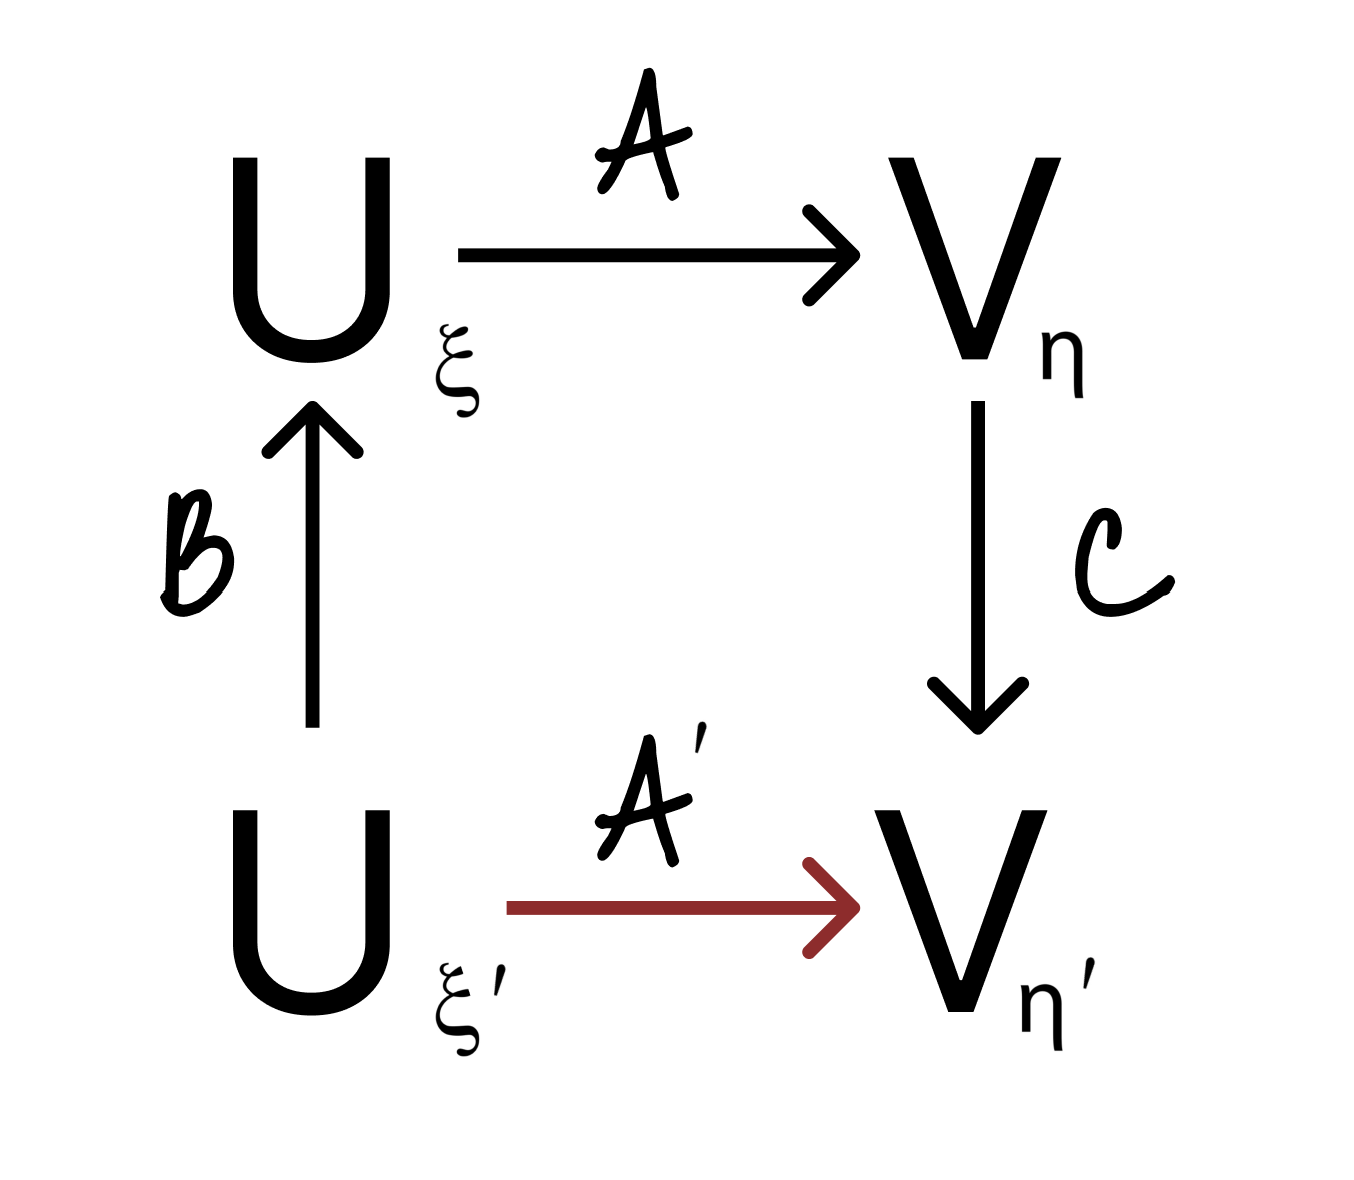
\includegraphics[width = 5cm]{assets/7_2_1.png}
\end{center}
    Воспользуемся данным рисунком, чтобы понять происходящее. Мы хотим найти матрицу $\mathcal{A}'$. Для этого, заметим, что преобразование $\mathcal{A}'$, это преобразование $\mathcal{B}$, потом примененное к нему преобразование $\mathcal{A}$, а после этого применненое к нему преобразование $\mathcal{C}$. То есть:
    $$\mathcal{A}'=\mathcal{C}\mathcal{A}\mathcal{B}$$

    Заметим, что матрица $\mathcal{B}$, это матрица перехода из $\xi$ в $\xi'$. Это так потому что у нас просто меняется базис (про саму матрицу перехода см. одноименный раздел). Матрица $\mathcal{C}$, это $T_{\eta' \rightarrow \eta}$. Откуда, исходя из двух утверждений сверху:
    $$A' = T_{\eta' \rightarrow \eta} A T_{\xi\rightarrow \xi'}\Rightarrow A' = T^{-1}_{\eta \rightarrow \eta'} A T_{\xi\rightarrow \xi'}$$ 

\hfill Q.E.D.
%todo

\deff{Следствие:} $A \in End(V)$. $e,e'$ базисы V. $A' = T^{-1}AT$, где $T = T_{e \to e'}$.

\deff{def:} квадратные матрицы $A$ и $B$ называются подобными, если $\exists$ невырожденная матрица $C$, такая, что: $B = C^{-1}AC$.

\textbf{Замечание:} матрицы линейного оператора в разных базисах подобны (см. следствие выше).

\subsection{Инварианты линейного отображения.}

\deff{Инвариатность} называется некоторое свойство объекта, которое не меняется при определенных действиях и преобразованиях.

$\mathcal{A}$ - линейное отображение. Ранг и дефект инварианты относительно выбора базиса.

Пусть $\mathcal{A} \in End(V)$. Пусть $e_1,\ldots, e_n$ базис $v$.

Как мы знаем, $\exists! D$ n-форма, такая что $D(e_1,\ldots e_n) = 1$. Тогда 
\deff{определитель} \deff{линейного оператора}:
$$\det \mathcal{A} := det(\mathcal{A}e_1,\ldots,\mathcal{A}e_n) = D(\mathcal{A}e_1,\ldots ,\mathcal{A}e_n)$$ 
\textbf{Замечание:} $\det \mathcal{A} = D(\mathcal{A}e_1,\ldots ,\mathcal{A}e_n) = D({A}e_1,\ldots ,{A}e_n) = \det A$ --- определение определителя линейного оператора и матрицы соотносятся.

\thmm{Теорема:}

$\forall\mathcal{A}  \in End(V), \det \mathcal{A} = \det A$.

\textbf{Доказательство:}

Возьмем $e = (e_1,\ldots, e_n)$ базис $V$. Тогда:
$$\mathcal{A}  \xleftrightarrow{\text{вз. однозначно}} A = (a_{ij})_{n\times n}$$
$$\det \mathcal{A} = D(\mathcal{A}e_1,\ldots,  \mathcal{A} e_n)  = D(\sum\limits_{i=1}^na_{i1}e_{i_1},\ldots,\sum\limits_{i=1}^n a_{in}e_{i_n}) =$$$$\xLeftrightarrow{\text{тк $D$ - $n$ форма}}\det \mathcal{A}=\sum\limits_{i_1=1}^n\ldots \sum\limits_{i_n=1}^n a_{i_11}\cdot\ldots\cdot a_{i_nn} D(e_{i_1}\ldots,e_{i_n}) = $$
$$= \sum\limits_{\sigma \in S_n}  a_{i_11}\cdot\ldots\cdot a_{i_nn} \cdot (-1)^{\varepsilon(\sigma)}D(e_1,\ldots,e_n)=\det A$$

\hfill Q.E.D.

\textbf{Замечание:} $A$ и $B$ подобные матрицы, то $\det A = \det B$. 

\textbf{Замечание:} $\det \mathcal{A}$ \uline{инвариант} линейного оператора, он не зависит от базиса.

\textbf{Следствие 1:} $\forall n$ - форма $f$ на $V$, $\forall \mathcal{A} \in End(V)$:
$$\forall \xi_1,\ldots, \xi_n \in V: f(\mathcal{A}\xi_1.\ldots, \mathcal{A}\xi_n) =\det A f(\xi_1,\ldots, \xi_n)$$
\textbf{Доказательство:}

Возьмем $e = (e_1,\ldots,e_n)$ базис $V$. $\mathcal{A} \xleftrightarrow{e}A$. Это значит, что мы берем матрицу линейного оператора в данном базисе.
$$f(\mathcal{A}e_1.\ldots, \mathcal{A}e_n) \overset{\text{из доказательства теоремы}}{=}\det Af(e_1,\ldots,e_n)$$
На самом деле $\alpha = f(e_1.\ldots,e_n)$, поэтому:
$$\forall \xi_1,\ldots,\xi_n : g(\xi_1,\ldots,\xi_n):= f(\mathcal{A}\xi_1,\ldots, \mathcal{A} \xi_n)$$
Заметим, что $g$ - полилинейное, тк $f$ полилин. и $\mathcal{A}$ - лин. отобр. Также $g$ - антисим, тк $f$ - антисим. Откуда $g$ - $n$-форма. Заметим интересный факт:
$$g(e_1,\ldots,e_n) = f(\mathcal{A}e_1,\ldots,\mathcal{A}e_n) = \det A \cdot f(e_1,\ldots,e_n)$$
Откуда:
$$ g(\xi_1,\ldots,\xi_n)= g(e_1,\ldots,e_n) D(\xi_1,\ldots,\xi_n) = \det A  \cdot \alpha D(\xi_1,\ldots,\xi_n) = \det A \cdot f(\xi_1,\ldots,\xi_n)$$
\hfill Q.E.D.

\textbf{Замечание:} Мы можем вывести 9-ое свойство определителя по-другому. Пусть $\mathcal{A} = A_{n\times n}$ --- линейный оператор умножения.
$f = D$, $B_j \in K^n$. Тогда:
$$det(AB_1,\ldots, AB_N) = \det A \cdot \det B $$
\textbf{Следствие 2:}
$\mathcal{A},\mathcal{B} \in End(V) \Rightarrow \det(\mathcal{A} \mathcal{B}) = \det \mathcal{A} \cdot \det \mathcal{B}$

\textbf{Доказательство:}

Пусть $e$ - базис $V$. Тогда $\mathcal{A} \xleftrightarrow{e}A, \mathcal{B}\xleftrightarrow{e}B$. Также $\mathcal{A}\mathcal{B} \xleftrightarrow{e}AB$ по свойству. Откуда:
$$\det \mathcal{A}\mathcal{B} = \det(AB) = \det A \cdot \det B = \det \mathcal{A} \cdot \det\mathcal{B}$$
\hfill Q.E.D.

\textbf{Следствие 3:} $\mathcal{A} \in Aut(V) \Leftrightarrow \det A \neq 0$. Причем $\det \mathcal{A}^{-1} = \cfrac{1}{\det \mathcal{A}}$

\textbf{Доказательство:}
$$\mathcal{A} \in Aut(V) \Leftrightarrow \begin{cases}
    \mathcal{A} \in End(V) \\
    \text{изоморфизм}
\end{cases} \Leftrightarrow \begin{cases}
    \mathcal{A} \in End(V)\\
    def \mathcal{A} = \dim \ker \mathcal{A} = 0
\end{cases} \Leftrightarrow $$
$$\Leftrightarrow\begin{cases}
    \mathcal{A}\in End(V) \\
    rg \mathcal{A} = n
\end{cases} \Leftrightarrow \begin{cases}
    \mathcal{A} \xleftrightarrow{e} A,\det A \neq 0 \\
    \rg A = n
\end{cases}$$
Мы знаем, что существует $\mathcal{A}^{-1}$. А также $\mathcal{A}\cdot \mathcal{A}^{-1}=\varepsilon$. Откуда по свойству 3 получаем, что $\det \mathcal{A}^{-1} = \cfrac{1}{\det \mathcal{A}}$

\hfill Q.E.D.

\textbf{Следствие 4:} $\det( \mathcal{A} \mathcal{A}^{-1})= 1 = \det  \mathcal{A} \cdot \det \mathcal{A}^{-1}$


Вспомним старое определение $tr A = \sum\limits_{i=1}^n a_{ii}$ - \emph{след матрицы}.

\thmm{Теорема (о tr подобных матриц)}

Если $A$ и $B$ подобны, то $tr A = tr B$.

\textbf{Доказательство:}

$A$ и $B$ подобны $\Leftrightarrow\exists C :B =C^{-1}AC$. Пусть $C^{-1} = S = (s_{ij})$. Откуда:
$$tr B = \sum\limits_{i=1}^n b_{ii} = \sum\limits_{i=1}^n \sum\limits_{j=1}^ns_{ij} (AC)_{ji} = \sum\limits_{i=1}^n \sum\limits_{j=1}^n \sum\limits_{k=1}^n s_{ij}\cdot a_{jk} \cdot c_{ki} = \sum\limits_{j=1}^n\sum\limits_{k=1}^n a_{jk}\sum\limits_{i=1}^nc_{ki}s_{ij}$$
Заметим, что $(CS)_{kj} = \delta_{kj}$, где $\delta_{kj}=\begin{cases}
    1, k=j\\
    0, k\neq j
\end{cases}$. Так что получаем, что 
$$tr B = \sum\limits_{i=1}^n a_{ii} = tr A$$
\hfill Q.E.D.

\textbf{Следствие:} $\forall \mathcal{A} \in End(V) \Rightarrow tr(A) = tr A'$, где $A$ и $A'$ матрицы оператора $\mathcal{A}$ в базисе $e$ и $e'$ соответственно.

\deff{def:} $\mathcal{A} \in End(V), tr \mathcal{A} = tr A$ --- \deff{след оператора}.

\textbf{Замечание:} след оператора инвариантен из следствия выше.

\deff{def:} Линейное подпространство $L \subset V$ называется \deff{инвариантным} относительно линейного оператора $\mathcal{A}\in End(V)$, если $\forall v \in L, \mathcal{A} v \in L$.

\thmm{Теорема 1:}

$L \subset V$ - линейное подпространство. $L$ - инвариантно относительно $\mathcal{A} \in End(V)$. Тогда $ \exists $ базис пр-ва $V$ матрица, такой что матрица оператора $\mathcal{A}$ в этом базисе будет иметь \emph{ступенчатый вид}, при этом размерность $A^1 = k \times k,  \, k = \dim L$.
$$A =\begin{pmatrix}
    A^1 & *\\
    \zero & A^2
\end{pmatrix}$$
\textbf{Доказательство:}

$L = \span (e_1,\ldots, e_k)$ - базис $L$.

Дополним базис $L$ до базиса $V$: $V = \span (e_1,\ldots, e_k, e_{k+1},\ldots,e_n)$.

Запишем матрицу $A$ по определению:

$$\forall e_i\in L:\mathcal{A}e_i \in L  \Rightarrow \mathcal{A}e_i = \sum\limits_{j=1}^ka_{ji}e_j \leftrightarrow A_i = \begin{pmatrix}
    a_{1i}\\
    \vdots\\
    a_{ki}\\
    0\\
    \vdots\\0
\end{pmatrix}$$ 
Откуда $A = \begin{pmatrix}
    a_{11}&\ldots&a_{1k} & * & \ldots & *\\
    \vdots&\ddots & \vdots &\vdots& \vdots & \vdots\\
      a_{k1}&\ldots &  a_{k1} &\vdots& \vdots & \vdots\\
      0&\ldots &  0 &\vdots& \vdots & \vdots\\
        0&\ldots &  0 &*& \ldots & *\\
\end{pmatrix} \Rightarrow A^1 = \begin{pmatrix}
     a_{11}&\ldots&a_{1k}\\
     \vdots&\ddots & \vdots\\
     a_{k1}&\ldots &  a_{k1} \\
\end{pmatrix}$

\hfill Q.E.D.

\thmm{Теорема 2:}

$V = \bigoplus\limits_{i=1}^m L_i$, $L_i$ инвариантны отн. $\mathcal{A}$.
$\Rightarrow \exists$ базис пр-ва $V$, такое что м-ца оператора $\mathcal{A}$ будет иметь блочно-диагональный вид: 
$$
\begin{pmatrix}
    A^1 &\ldots&\ldots& \zero\\
    \vdots &A^2&\ldots& \vdots\\
    \vdots  & \vdots &\ddots& \vdots\\
    \zero & \ldots &\ldots& A^n
\end{pmatrix}$$
\textbf{Доказательство:}

Пусть базис $V \overset{\text{по эквив. условию $\oplus$}}= $ объединение базисов $L_i$.
$$L_i = \span(e_1^i,\ldots ,e_{k_i}^i),\dim L_i = k_i$$
Построим матрицу по определению. Не трудно заметить, что для каждого $L_i$ из доказательства прошлой теоремы, все кроме соотв. строчек для $L_i$ будет зануленно.

\hfill Q.E.D.

\textbf{Замечание:} $A_i \leftrightarrow A|_{L_i}\in End(L_i)$.


\thmm{Теорема 3.}

$V = \bigoplus\limits_{i=1}^m L_i$, $L_i$ инвариантны отн $\mathcal{A} \Rightarrow \Im\mathcal{A} = \bigoplus\limits_{i=1}^m  \Im \mathcal{A}|_{L_i}$, где
$\mathcal{A}|_{L_i}\in L(L_i,V)$


\textbf{Доказательство:}
$$V = \bigoplus\limits_{i=1}^mL_i \xLeftrightarrow{\text{из т. об экв. опр. прямой суммы}} \forall v \in V: \exists! v = \sum\limits_{i=1}^mv_i, v_i \in L_i$$
$$\forall  v \in V: \Im \mathcal{A}\ni\mathcal{A}v = \mathcal{A}\sum\limits_{i=1}^m v_i =\sum\limits_{i=1}^m\mathcal{A}v_i\in \Im A|_{L_i}$$
Тогда всё, что нам осталось проверить это то, что наши пространства дизъюнкты. Но, если присмотреться к тому, что у нас написано, то у нас для любого вектора из $\Im \mathcal{A}$ существует лишь одно разложение через $\Im A|_{L_i}$, что соответствует эквивалентному определению прямой суммы.

\hfill Q.E.D.
\subsection{Собственные числа и собственные векторы лин. оператора}

$\lambda \in K $ называется \deff{собственным числом} $\mathcal{A} \in End(V)$, если $\exists v \in V,v\neq 0$. $\mathcal{A} v = \lambda v$. Такой $v$  называют \deff{собственным вектором} собственного числа $\lambda$.

$$\lambda \in K: \begin{cases}
    \mathcal{A} v =\lambda v\\
    v\neq 0
\end{cases} \Leftrightarrow \begin{cases}
    (A-\lambda \varepsilon)v = 0 \\
    v \neq 0
\end{cases} \Leftrightarrow\begin{cases}
    v \in \ker (A-\lambda\varepsilon)\\
    v\neq 0
\end{cases}\Leftrightarrow $$

$\Leftrightarrow v$ собственный вектор собственного числа  $\lambda$.

$V_{\lambda} = \ker(A-\lambda\varepsilon) $ %написать это в 2 строчки
--- \deff{собственное подпространство} $\mathcal{A}$ соответств. с.ч. $\lambda$. Это  {мн-во всех с.в. $V$, отвечающим с.ч. $\lambda$  и нулевой вектор}.

$\gamma(\lambda) = \dim V_{\lambda}$ --- \deff{геометрическая кратность}.

\textbf{Свойства:}
\begin{enumerate}
    \item $V_{\lambda}$ инвариантно относительно $(\mathcal{A}-\lambda \varepsilon)$.
    \item $V_{\lambda}$ инвариантно относительно $\mathcal{A}$.
    \item $\gamma(\lambda)$ инвариант относительно базиса.
\end{enumerate}

\textbf{Условие существования с.ч.:} \\
$\lambda \in K_{\mathcal{A}}$ - с.ч., $v$ - с.в. $\Leftrightarrow \ker (A-\lambda\varepsilon)$ нетривиально $ \Leftrightarrow def(\mathcal{A} - \lambda\varepsilon) \ne 0 \Leftrightarrow rg(\mathcal{A} - \lambda\varepsilon) \ne n \Leftrightarrow \det(\mathcal{A} - \lambda \varepsilon) = 0$

Тк определитель линейного оператора  инвариантен, то:
$$\det(\mathcal{A} - \lambda \varepsilon) = 0 \Leftrightarrow \det({A} - \lambda E) = 0$$
\deff{def:} $\chi(t) = \det (\mathcal{A} - t\varepsilon)$ - \deff{характеристический многочлен} оператора $\mathcal{A}$.

Т.к. $\det$ оператора инвариантен $\chi(t) = \det (A - tE)$, где $A$ - матрица линейного оператора $\mathcal{A}$ в некотором базисе.
$$\chi(t) =\begin{vmatrix}
    a_{11} -t & a_{12} & \ldots & a_{1n} \\
    a_{21} & a_{22}-t & \ldots & \vdots\\
    \vdots & \vdots & \ddots & \vdots\\
    a_{n1} & a_{n2} & \ldots & a_{nn}-t
\end{vmatrix} = (-1)^{n}\cdot t^n + (-1)^{n-1}(tr At^{n-1}) + \ldots + \det A$$
По теореме Виета:
$\begin{cases}
t_1 +\ldots+t_n = tr A\\
t_1\cdot \ldots \cdot t_n = \det A
\end{cases}$
Заметим, что $\lambda$ с.ч. $\mathcal{A} \Leftrightarrow\begin{cases}
    \lambda \in K\\
    \chi(\lambda) = 0 \text{ - корень хар. мн.}
\end{cases}$

\textbf{Замечание.} Если все корни хар. мн. $\in K \Rightarrow$ $\begin{cases}
\lambda_1 +\ldots+\lambda_n = tr A\\
\lambda_1\cdot \ldots \cdot \lambda_n = \det A
\end{cases}$

\deff{def:} \deff{Спектром} оператора $\mathcal{A}$ называется множество $\{ (\lambda$, $\alpha(\lambda)) \}$, 
$\alpha(\lambda)$ - кратность $\lambda$ лин. оператора в хар. уравнении (\emph{алгебраическая кратность}). Спектр это множество пар.

\deff{def:} \deff{Простой спектр} --- все кратности -  единички.


\thmm{Теорема 1:}

$\forall \mathcal{A}\in End(V)$. $\forall \lambda$ с.ч. $\mathcal{A} : 1\leq \gamma(\lambda)\leq \alpha(\lambda)$

\textbf{Доказательство:}

$\lambda$ с.ч. $\mathcal{A} \Leftrightarrow \ker(\mathcal{A}-\lambda \varepsilon)= V_{\lambda}$ не тривиально $\Leftrightarrow \gamma_1=\dim V_\lambda\geq 1$.

Пусть $\dim V_{\lambda} = \gamma$, $V_{\lambda}$ инвариантно относительно $\mathcal{A} \Rightarrow$ по т-ме 1 об инв. подпр. существует $V$ такой, что матрица оператора $\mathcal{A}$ будет иметь ступенчатый вид:
$$A =\begin{pmatrix}
    A^1 & *\\
    \zero & A^2
\end{pmatrix}$$
$$\dim A^1 = \gamma \times \gamma,V = \span(e_1,\ldots, e_{\gamma},e_{\gamma+1},\ldots,e_{n})$$

При построении матрицы оператора $\mathcal{A}$:

$\mathcal{A}e_i = \lambda e_i \leftrightarrow A_i = \begin{pmatrix}
    \vdots \\
    0\\
    \lambda\\0\\\vdots
\end{pmatrix}$ - $\lambda$ - на $i$-ой строчке. Немного распишем:

$$\chi(t) = \det(A-tE) =\begin{vmatrix}
    A^1-tE_{\gamma\times\gamma} & *\\
    \zero & A^2 -tE_{(n-\gamma)\times(n-\gamma))}
    \end{vmatrix} \overset{\text{по 6-ому св-ву опр}}=$$
    
    
    $$= |A^1-tE||A^2-tE|=\chi_{A^1}(t)\cdot \chi_{A^2}(t)=(\lambda-t)^\gamma\chi_{A_2}(t) \Rightarrow$$
    $ \Rightarrow \lambda $ корень $\chi(t)$, причем кратность $\geq \gamma$, т.к $\lambda$ может оказаться корнем $\chi_{A^2}$

\hfill Q.E.D.


\thmm{Теорема 2:}

$\lambda_1,\lambda_2,\ldots,\lambda_n$ попарно различные с.ч $\mathcal{A}$, $v_1,\ldots,v_n$ соответ. с.в.

$\Rightarrow v_1,\ldots,v_n$ --- лин. независимы.

\textbf{Доказательство:}

Докажем по индукции:

\textbf{База} $m = 1: \lambda_1,v_1 \Rightarrow$ лин. незав.

\textbf{ИП}: Пусть верно для $m$, докажем для $m+1$:

\uline{От противного:} Пусть $\lambda_1,\ldots,\lambda_m,\lambda_{m+1}$ попарно различные собственные числа. 

$v_1,\ldots,v_m$ - линейно независимы по ИП. $v_1,\ldots,v_m,v_{m+1}$ - линейно зависимы. Откуда: $v_{m+1}=\sum\limits_{i=1}^m \alpha_i v_i$. С одной стороны:
$$\mathcal{A} v_{m+1} = \lambda_{m+1} v_{m+1} = \lambda_{m+1}\sum\limits_{i=1}^m\alpha_iv_i$$
C другой стороны:
$$\mathcal{A} v_{m+1} =\mathcal{A}\sum\limits_{i=1}^m \alpha_i  v_i  =\sum\limits_{i=1}^m \alpha_i \mathcal{A} v_i = \sum\limits_{i=1}^m\alpha_i \lambda_i v_i$$
$$\sum\limits_{i=1}^m(\lambda_{m+1}-\lambda_i)a_i v_i = 0$$

% у меня в конспекте такое доказательство с лекции, которое показалось понятнее:
% все v_i не нули, все разности лямбд тоже не нули
% тогда все альфы нули, но тогда v_{m + 1} = 0, противоречие
Но мы знаем, что $v_1,\ldots,v_m$ линейно независимы. Откуда эта линейная комбинация тривиальна, но с другой стороны, она такой быть не может, потому что $\exists \alpha_i\neq 0$, для которого $v_i$ не равен нулю, а так же, исходя из того что искомые с.ч. попарно различны, то $\lambda_{m+1}-\lambda_i\neq 0$. Откуда комбинация нетривиальна. 

Противоречие.

\hfill Q.E.D.

\textbf{Следствие:} $\lambda_1, \ldots,\lambda_m$ попарно различные с.ч. $\mathcal{A} \Rightarrow \bigoplus\limits_{i=1}^m V_{\lambda_i}$, т.е $V_{\lambda_i}$ дизъюнктны.

\textbf{Доказательстсво:}
$$\zero = v_1 + \ldots+ v_m, v_i \in V_{\lambda_i}$$
Если в сумме какой-то из векторов ненулевой, то это собственный вектор, а собственные вектора для различных с.ч. линейно независимы. Противоречие. Откуда все вектора в сумме нулевые, откуда подпространства дизъюнктны.

\hfill Q.E.D.

\thmm{Теорема 3:}

$V = \bigoplus\limits_{i=1}^mL_i$, $L_i$ инвариантно относительно $\mathcal{A} \in End(V)$

$\Rightarrow \chi(t) = \det(\mathcal{A} - t\varepsilon) = \prod\limits_{i=1}^m\chi_{\mathcal{A}_i}(t) $.

\textbf{Доказательство:}

Смотрим теорему 3 об инв. подпр. Матрица A - блочно-диагональная:
$$A = \begin{pmatrix}
    A^1 &\ldots&\ldots& \zero\\
    \vdots &A^2&\ldots& \vdots\\
    \vdots  & \vdots &\ddots& \vdots\\
    \zero & \ldots &\ldots& A^n
\end{pmatrix}$$
  Тогда $\chi(t) = \det(A-tE) \overset{\text{по 6-ому свойству опр.}}= \prod\limits_{i=1}^m \det(A^i-tE) = \prod\limits_{i=1}^m \chi_{A_{L_i}}(t) $

\hfill Q.E.D.


\subsection{Оператор простой структуры (о.п.с). Проекторы. Спектральное разложение. Функция от диагонализированной матрицы.}

$\mathcal{A} \in End(V)$ называется \deff{оператором простой структуры} (о.п.с), если $\exists$ базис пространства $V$ такой, что матрица оператора $\mathcal{A}$ в этом базисе имеет диаг. вид.
$$\Lambda = diag(\lambda_1,\ldots,\lambda_n)=\begin{pmatrix}
    \lambda_1 & \ldots & 0 \\
    \vdots & \ddots & \vdots\\
    0 & \ldots &\lambda_n
\end{pmatrix}$$

Заметим, что в таком случае  собственные числа  оператора $\mathcal{A}$ будут $\lambda_i$, а так же собственные вектора этих чисел - соотв. столбики (легко проверить умножением). Отсюда  все корни характ. многочлена  $\chi \in K \Leftrightarrow \sum\limits_{\lambda \text{-с.ч.} \mathcal{A}}\alpha(\lambda) = n = \dim V$.



\thmm{Теорема:}

$\forall \mathcal{A} \in End(V)$, если  $\sum\limits_{\lambda \text{-с.ч.} \mathcal{A}} \alpha(\lambda)= n$, то тогда:
$$\mathcal{A} \text{ - о.п.с} \Leftrightarrow \forall\lambda \text{ - с.ч }: \gamma(\lambda) = \alpha(\lambda) \Leftrightarrow \sum\limits_{\lambda \text{-с.ч.} \mathcal{A}}\gamma(\lambda) = n = \dim V$$
\textbf{Доказательство:}

$ \sum\limits_{\lambda \text{-с.ч.} \mathcal{A}} \alpha(\lambda) = n \Leftrightarrow$ все корни $\chi \in K$, откуда $\mathcal{A}$ -  о.п.с.

$\mathcal{A}$ о.п.с. $\Leftrightarrow \exists$ базис $V$ такой, что матрица диагональна $\Leftrightarrow$ $$\Leftrightarrow V = \bigoplus\limits_{\lambda - \text{с.ч.}}V_{\lambda} \Leftrightarrow \sum\limits_{\lambda - \text{с.ч.}}\gamma(\lambda) = n =\dim V$$
\hfill Q.E.D.

\textbf{Следствие.} Если все корни характ. многочлена $\in K$, а также все $\alpha(\lambda)=1$ (спектр простой), то $\mathcal{A}$ - о.п.с.

\deff{def:} $A_{n\times n}$ называется \deff{диагонализируемой}, если  она подобна диагональной.

\thmm{Теорема (критерий диагональности матрицы $A$)}

\sout{это перепишетcя}

$A$ подобна диагональной $\Leftrightarrow$ матрица о.п.с $\mathcal{A}$ в нек. базисе

\textbf{Доказательство:}

\begin{itemize}
    \item  \fbox{\(\Rightarrow\)}
    
    Пусть $A$ - диагонализируемая $\Leftrightarrow$ подобна диагональной $\Leftrightarrow$ $\exists$ невырожд T: $T^{-1}AT=\Lambda=diag(\lambda_1,\ldots,\lambda_n)$. $V$ - линейное пространство над полем $K$. $e = (e_1,\ldots,e_n)$ - базис V.

    Пусть $A$ - матрица в базисе $e$. Тогда $Ae_j = \sum\limits_{i=1}^na_{ij}e_i$.$v =(v_1,\ldots,v_n)$ - базис.\\Откуда $v_1,\ldots,v_n = (e_1,\ldots,e_n)T_{e\rightarrow v} \Rightarrow \mathcal{A}\xleftrightarrow{v} A' = T^{-1}AT=\Lambda$ 
    \item \fbox{\(\Leftarrow\)}
    $\mathcal{A}$ о.п.с, $A$ - матрица в некотором базисе $e= (e_1,\ldots,e_n)$.
    Возьму $v_1, ..., v_n$ - базис V, где $v_i$ - собственный вектор $\mathcal{A}$. Заметим, что так как $\mathcal{A}$ о.п.с, то такой базис существует

   Теперь давайте возьмем матрицу перехода из $T_{e\rightarrow v}$. Тогда $\mathcal{A}\xleftrightarrow{v} A' = T^{-1}AT=\Lambda \Rightarrow A$ подобна диагональной   

    \hfill Q.E.D.
\end{itemize}
   
\textbf{Алгоритм поиска диагонального представления матрицы подобной диагональной:}
\begin{enumerate}
    \item найти спектр: если все корни $\chi \in K $, переходим к п2.
    \item найти все $\gamma(\lambda)$, если $\forall \lambda$ с.ч $\gamma(\lambda) = \alpha(\lambda)$, то перейти к п3.
    \item $T_{\text{кан.}\rightarrow v} = (v_1,\ldots,v_n)$ $T^{-1}AT = \Lambda$
\end{enumerate}







\deff{def:} $V = \bigoplus\limits_{i=1}^mL_i$. По теореме об равносильных условиях прямой суммы: 
\\$\forall v\in V: \exists! v = \sum\limits_{i=1}^mv_i, \text{где } v_i \in L_i$. Возьму $P_i \in  End(V)$,  такие, что $P_i \cdot v = v_i \in L_i$.\\ Тогда такие $P_i$ назовем \deff{операторами проектирования} на подпр-во $L_i$.



\textbf{Свойства операторов проектировния:}

\begin{enumerate}
  \item $\Im P_i = L_i$, \,
    $\ker P_i = \bigoplus\limits_{j\neq i}L_j $
    \item $P_i P_j = \zero$
    \item$\sum\limits_{i=1}^m P_i = \varepsilon$  %todo: возможно более подробно расписать
    \item $P_i^2 = P_i, (P_j^k = P_j , \text{где } k \in  \mathbb{N} )$ - \deff{идемпотентность}
\end{enumerate}

Они все тривиальны

\textbf{Утверждение.} Возьму множество операторов: $\{P_i\}_{i=1}^m$, $P_i \in End(V)$. 

Пусть они удовлетворяют свойствам 2,3 $\Rightarrow V  = \bigoplus\limits_{i=1}^m\Im P_i$. $P_i$ это проектор на $L_i$.

\textbf{Доказательство:}

Мы знаем, что $P_i P_j = \zero$, для $i \neq j$, а также $\sum\limits_{j=1}^m P_i = \varepsilon$. Откуда получаем, что:
$$ P_i = P_i \varepsilon = P_i\sum\limits_{j=1}^m P_j = \sum\limits_{j=1}^m P_j P_i = P_i^2$$ 
А это значит, что $\forall v \in V: v = \varepsilon v = \sum\limits_{i=1}^m P_iv \Rightarrow V = \sum\limits_{i=1}^m\Im P_i$.

Осталось показать единственность разложения нуля:
$$\zero = \sum\limits_{i=1}^mv_i = \sum\limits_{i=1}^m P_i w_i \text{, где } w_i \in V$$
$$P_j \zero = \zero = P_j \sum\limits_{i=1}^nP_iw_i = \sum\limits_{i=1}^n P_iP_j w_i = P_jw_j = v_j$$

$\Rightarrow v_j = \zero, \forall j= 1 \dots m \text{ }$
$\Rightarrow \text{дизъюнк. }\Rightarrow \bigoplus \Im P_i$

  \hfill Q.E.D.



\textbf{Замечание:} Из определения проекторов следует, что они существуют и определены  однозначно для данной прямой суммы.

\thmm{Теорема (спектральное разложение о.п.с)}

Дан $\mathcal{A} \in End(V)$. Тогда выполнено:

1) $\mathcal{A}$ --- о.п.с. $\Rightarrow$ $\mathcal{A} = \sum\limits_{\text{$\lambda$ - с.ч.}} \lambda P_{\lambda}, P_\lambda$ --- проектор на $V_\lambda$ $\forall \text{ с.ч. } \lambda$.

Такое разложение называется \deff{спектральным}.

2) $V =  \bigoplus\limits_{i=1}^m L_i$, $P_i$ проекторы на $L_i$. $\mathcal{A} = \sum\limits_{j=1}^m \lambda_iP_i \Rightarrow \mathcal{A} \text{ о.п.с, }\lambda_i \text{ с.ч.}$

$\Im P_i = L_i = V_{\lambda} \text{(соотвест. подпр-во)}$

\textbf{Доказательство:}

1) $\mathcal{A}$ о.п.с $\Leftrightarrow V = \bigoplus\limits_{\lambda \text{ - с.ч}} V_{\lambda}$. Возьму $P_\lambda$ проекторы на $V_\lambda$ (исходя из определения -они существуют) Тогда давайте воспользуемся определением:
$$\forall v \in V:  \exists! v =\sum\limits_{\lambda \text{ - с.ч}}v _{\lambda}, \text{где } v_\lambda \in V_\lambda:\mathcal{A}v = \mathcal{A}(\sum\limits_{\lambda} v_\lambda) = \sum\limits_{\lambda}\mathcal{A}v_{\lambda}  = \sum\limits_{\lambda }\lambda v_\lambda =\sum\limits_{\lambda}\lambda P_\lambda v $$

Откуда уже крайне очевидно получаем, что $  \mathcal{A} = \sum\limits_{\lambda}\lambda P_\lambda$.

2) $V=  \bigoplus\limits_{i=1}^m L_i$. Откуда по определению: $\forall v  \in V: \exists! v=\sum\limits_{i=1}^m v_i \in L_i = \Im P_i$, $v_i \ne 0$. Тогда
$$\mathcal{A} v_i=(\sum\limits_{j=1}^m \lambda_j P_j)v_i=(\sum\limits_{j=1}^m \lambda_j P_j)P_i v= v \sum\limits_{j=1}^m \lambda_j  P_j P_i$$
Теперь вспомним свойство, что при умножении двух различных операторов мы получаем $\zero$. Поэтому на самом деле наша сумма равна:
$$v \sum\limits_{j=1}^m \lambda_j  P_j P_i = v  \lambda_i  P_i P_i = v \lambda_i P _i = \lambda_i v_i$$
Хорошо, теперь вспомним, что изначально это было равно $\mathcal{A}v_i$. поэтому $\mathcal{A}v_i =  \lambda_iv_i$, откуда получаем, что $v_i$ с.в. $\mathcal{A}$ отвечающий с.ч. $\lambda_i$.

Откуда получаем, что  наше подмножество $ V_{\lambda_i} \supseteq \Im P_i$ (потому что любой $v \in \Im P_i$ --- собственный вектор).

Вспомним, что: $V = \bigoplus\limits_{i=1}^m \Im P_i \subseteq  \bigoplus\limits_{i=1}^m V_{\lambda_i}$, а как мы знаем $\bigoplus\limits_{i=1}^m V_{\lambda_i} \subseteq V$. Откуда, я получаю, что:
$$\bigoplus\limits_{i=1}^m \Im P_i = \bigoplus\limits_{i=1}^m V_{\lambda_i} \xRightarrow{\text{так как $P_i \subseteq V_{\lambda_i}$}}  \Im P_i = V_{\lambda_i}$$


  \hfill Q.E.D.


\thmm{Следствие (спектральное разложение диагонализируемой матрицы)}

$A$ диагонализируема $\Leftrightarrow$ $\exists! \{P_i\}_{i=1}^m$, такое, что  $P_i \cdot P_j = \zero$, $i\neq j$
и $\sum\limits_{i=1}^m P_i=E$,
$A = \sum\limits_{i=1}^m\lambda_iP_i$

\textbf{Доказательство:} 

Очевидно следует из теоремы: 

$A$ диагонализируема $\iff$ матрица $\mathcal{A}$ о.п.с. Либо можно считать  $A=\mathcal{A}$ о.п.с. 	$\in End (K^n)$

  \hfill Q.E.D.

\textbf{Замечание.} Матрица $A$ подобна диагональной, то у нее есть \uline{диагональное представление}:
$$T^{-1}AT = \Lambda = diag (\lambda_1 \dots \lambda_n), A = T \Lambda T^{-1}$$
А также у такой матрицы есть \uline{спектральное разложение}:
$$A=\sum\limits_{\lambda  \text{ c.ч.}}\lambda P_{\lambda}$$
Просьба не путать эти две формулы!

\textbf{СЕЙЧАС НАЧНЕТСЯ ЧТО-ТО СТРАШНОЕ}

\deff{def:} $A_k = (a_{ij}^k)_{n\times n}$ - последовательность матриц $n\times n$.

Обозначают так: $(A_k)_{k=1}^{\infty}$  --- \deff{последовательность матриц}.

Раз это последовательность, то давайте введем на ней вот такой предел:
$$A = \lim\limits_{n\rightarrow \infty} A_k = \forall i,j: a_{ij}=\lim\limits_{k\rightarrow \infty}a_{ij}^k$$
Для лучшего понимания этого мира смотрите на приведенный ниже пример:
$$\lim\limits_{k\rightarrow \infty}\left(
 \begin{matrix}
 (1+ \frac{2}{k})^k & \sqrt[k]{k} \\
 \frac{\sin \frac{\pi}k}{\frac1k} & \frac{1 - \cos \frac{\pi}k}{\frac{1}{k}}
 \end{matrix}
\right) = \left(
 \begin{matrix}
 e^2 & 1 \\
 \pi & 0
 \end{matrix}
\right)$$
\deff{def:} $a_n \in R: \sum\limits_{m=1}^{\infty}a_m = S \Leftrightarrow
\exists \lim\limits_{k \rightarrow \infty}\sum\limits_{m=1}^k a_m=S$, где $S_k =\sum\limits_{m=1}^k a_m $ --- \deff{частичная сумма ряда.}

А саму такую конструкцию понятно называют рядом. Теперь давайте немного притронемся к матану:

$\sum\limits_{m=0}^\infty c_mx^m$ - \deff{ряды Тейлора - Маклорена}. 

$x\in \mathbb{R}(\mathbb{C})$ --- их область определения, $|x| < R$ (или еще обозначается r) --- \deff{радиус сходимости}, $c_m \in \mathbb{R}(\mathbb{C})$. Причем эти $c$-шки на самом деле производные. (если интересно см. конспект по мат. анализу первый семестр)

\textbf{Рассмотрим пример:} Давайте разложим $e^x$, нам это позже понадобится:
$$e^x = \sum\limits_{n=0}^\infty\cfrac{1}{n!}x^n, |x| < + \infty$$
В таком случае $c_m = \cfrac{f^{(m)}(0)}{m!}$.

Пусть $f(x) = \sum\limits_{m=0}^\infty c_n x^n$. А давайте расширим на матрицы :)

\deff{def:} $A_{n\times n}: f(A) = \sum\limits_{m=0}^\infty c_mA^m$. Причем мы так же считаем частичные суммы и ищем их предел, но теперь просто ищем предел в матрицах.

Можно добавить параметр: $f(At) = \sum\limits_{m=0}^\infty c_mA^mt^m$.



\thmm{Теорема 1 (функция от диагонализируемой матрицы 1)}

Пусть $A$ --- подобна диагональной. А также нам дана $f(x) = \sum\limits_{m=0}^\infty c_m x^m, |x|<r$.

Тогда, если $\forall$ с.ч. $|\lambda|< r \Rightarrow \exists f(A)$ и $f(A) = T f(\Lambda) T^{-1}$, где
$f(\Lambda) = \begin{pmatrix}
    f(\lambda_1) & \ldots & 0\\
    \vdots & \ddots & \vdots \\
    0 & \ldots &f(\lambda_n)
\end{pmatrix}$

\textbf{Доказательство:}

Упрощу $\sum\limits_{m=0}^k    c_m A^m$. Мы знаем, что $A$ - подобна диагональной $ \Rightarrow A = T \Lambda T^{-1}$.  Тогда:
$$A^m = (T \Lambda T^{-1})^m = T \Lambda T^{-1} T \Lambda T^{-1} \ldots T \Lambda T^{-1} = T \Lambda^m T^{-1}$$
Теперь давайте подставим это в нашу сумму:
$$\sum\limits_{m=0}^k c_m A^m = \sum\limits_{m=0}^k c_mT \Lambda^m T^{-1} = T\left(\sum\limits_{m=0}^k c_m\Lambda^m\right)   T^{-1}$$
Теперь вспомним, что $\Lambda^n$ диагональня, поэтому занесем сумму внутрь матрицы и получим:
$$T\left(\sum\limits_{m=0}^k c_m\Lambda^m\right) T^{-1} = T \begin{pmatrix}
    \sum\limits_{m=0}^k c_m\lambda_1^m & \ldots & 0 \\
    \vdots  & \ddots & \vdots \\
    0 & \ldots & \sum\limits_{m=0}^k c_m\lambda_n^m
\end{pmatrix}T^{-1} =$$
Теперь вспомним, что $\forall$ с.ч. $|\lambda|< r$, поэтому для них мы можем применить формулу, откуда:
$$\lim\limits_{k\rightarrow\infty}\sum\limits_{m=0}^k    c_m A^m=\lim\limits_{k\rightarrow\infty} T \begin{pmatrix}
    \sum\limits_{m=0}^k c_m\lambda_1^m & \ldots & 0 \\
    \vdots  & \ddots & \vdots \\
    0 & \ldots & \sum\limits_{m=0}^k c_m\lambda_n^m
\end{pmatrix}T^{-1} =T \begin{pmatrix}
    f(\lambda_1) & \ldots & 0 \\
    \vdots  & \ddots & \vdots \\
    0 & \ldots &  f(\lambda_n)
\end{pmatrix}T^{-1}$$
  \hfill Q.E.D.

\thmm{Теорема 2 (функция от диагонализируемой матрицы, 2-я формула)}

Пусть $A$ --- подобна диагональной.

Тогда $A$ имеет спектральное разложение $\sum\limits_{\lambda \text{ - с.ч.}}\lambda P_\lambda$, где $P_{\lambda}$ --- проекторы. А также нам дана $f(x) = \sum\limits_{m=0}^\infty c_m x^m, \quad |x|<r$.

Тогда, если $\forall$ с.ч. $|\lambda|< r$, то $\exists f(A)$, а так же $f(A) = \sum\limits_{\lambda \text{ - с.ч.}}f(\lambda)P_\lambda$.

\textbf{Доказательство:}

$A^m = (\sum\limits_{\lambda }\lambda P_{\lambda})^m = \sum\limits_{\lambda}\lambda P_{\lambda}\sum\limits_{\mu}\mu P_{\mu} \ldots \sum\limits_{\xi}\xi P_{\xi}$

А теперь вспомним свойства проекторов. Когда я умножаю два разных проектора, я получаю ноль, откуда:
$$A^m = \sum\limits_{\lambda}\lambda P_{\lambda}\sum\limits_{\mu}\mu P_{\mu} \ldots \sum\limits_{\xi}\xi P_{\xi} = \sum\limits_{\lambda}\lambda^m P_{\lambda}^m = \sum\limits_{\lambda}\lambda^m P_\lambda$$
Значит: $\sum\limits_{m=0}^k c_m A^m =\sum\limits_{m=0}^k c_m  \sum\limits_{\lambda}\lambda^m P_\lambda =  \sum\limits_{\lambda}P_{\lambda} \sum\limits_{m=0}^k\lambda^m c_m $.  Теперь если я возьму предел, то я получу то, что мне нужно, потому что каждая лямбда $<r$, и поэтому я могу вместо них подставить $f(\lambda)$.

  \hfill Q.E.D.
\\

\deff{Экспонента:}

А теперь давайте возьмем все $c=1$,  а также вспомним, что мы можем протаскивать с собой параметр. Поэтому у нас получается новая формула:

$f(A) =\lim\limits_{k\rightarrow\infty}\sum\limits_{m=0}^k    t^mA^m$, а теперь вспомним наше разложение $e$-шки. А это именно оно и есть! Поэтому получаю:
$$e^{At}=f(At) =\lim\limits_{k\rightarrow\infty}\sum\limits_{m=0}^k  t^mA^m$$

Или:

$$e^{At} = T \begin{pmatrix}
    e^{\lambda_1t} & \ldots & 0 \\
    \vdots &\ddots& \vdots\\
    0 & \ldots & e^{\lambda_nt}
\end{pmatrix} T^{-1} = \sum\limits_{\text{$\lambda$ - с.ч.}} e^{\lambda t}P_{\lambda}$$


\textbf{Свойства:}
\begin{enumerate}
    \item  $(e^{At})' = Ae^{At} = e^{At}A$.

    \item $e^{(A_1+A_2)t}=e^{A_1t}\cdot e^{A_2t}$
    \item $e^{\zero t} = E$
\end{enumerate}

\deff{Обратная:}

$A$ - подобна диагональной 
$\forall $ с.ч. $\lambda \neq 0 \Rightarrow \exists A^{-1} = T\begin{pmatrix}
    \cfrac{1}{\lambda_1} & \ldots & 0 \\
    \vdots &\ddots& \vdots\\
    0 & \ldots &\cfrac{1}{\lambda_n}
\end{pmatrix} T^{-1}$

\textbf{Свойства:}
\begin{enumerate}
    \item $A^{-1} = \sum\limits_{\lambda \text{ - c. ч}}\cfrac{1}{\lambda}P(\lambda)$
    \item $AA^{-1}=T \Lambda T^{-1}T \Lambda^{-1} T^{-1} = E$
    \item $AA^{-1}=(\sum \mu P_{\mu})(\sum \frac{1}{\lambda}P_{\lambda})= \sum\limits_{\lambda} \lambda \frac{1}{\lambda}P_{\lambda} = E$
\end{enumerate}

\deff{Корень:}

Если $A$ подобна диагональной и $\forall$ с.ч. $\lambda \geq 0$, то взяв $m \in \mathbb{N}, m \geqslant2$ мы можем ввести:
$$\sqrt[m]{A} = T\begin{pmatrix}
    \sqrt[m]{\lambda_1} & \ldots & 0 \\
    \vdots &\ddots& \vdots\\
    0 & \ldots &\sqrt[m]{\lambda_n}
\end{pmatrix}T^{-1}\text{, полагая }\sqrt[m]{\lambda}\geqslant0$$
\textbf{Спектральное представление:}
$\sqrt[m]{A}= \sum\limits_{\lambda \text{  c. ч.}} \sqrt[m]{\lambda} P_{\lambda}$.


\subsection{Комплексификация вещ. лин. пр-ва. Продолжение вещественного линейного оператора}

Давайте посмотрим какие линейные операторы мы уже изучили: 


Пусть $\mathcal{A} \in End(V) \xleftrightarrow{e} A $, $\chi(t)$ --- корни характеристического многочлена. Он может быть:

\begin{enumerate}
    \item Все корни $\in K$. $\sum\limits_{\lambda \text{ - с.ч}}\alpha(\lambda) = n  = \dim V$
    \begin{itemize}
        \item $\exists$ базис $V$ из $v_{\lambda} $: $\,\,\forall \lambda:\,\,\alpha(\lambda)=\gamma(\lambda) \iff$ диагонализируема.
        \item $\not \exists $ базис $V$ из $v_{\lambda} \,\,$: $\exists $ с.ч. $\lambda$: $\,\, \gamma(\lambda) < \alpha(\lambda) \iff A$ жорданова форма.
    \end{itemize}
    \item Не все корни $\in K$. В таком случае вещ. $V$ комплексифицируют.
\end{enumerate}


\deff{def:} $V$ --- линейное пространство над $\mathbb{R}$ (вещ. лин. пр-во)
$$\forall x,y \in V \Rightarrow  z = x+iy \in V_{\mathbb{C}} \quad V_{\mathbb{C}} = \{ z = x+yi \bigm| \forall x,y \in V\}$$

Назовем $V_{\mathbb{C}}$ \deff{комплексификацией} $V$.

Покажем некоторые \textbf{свойства:}
\begin{enumerate}
    \item $\zero \in V \leftrightarrow \zero + i\zero = \zero \in V_{\mathbb{C}}$ - существование нуля 
     \item $x \in V \leftrightarrow x +i\zero = x \in V_c$, $V \subset V_{\mathbb{C}}$ --- говорим, что $V\subseteq  V_{\mathbb{C}}$ 
    \item $\forall z = x + iy$ существует обратное: $-x+i(-y)$
\end{enumerate}

Заметим, что в таком случае $V_\mathbb{C}$ ---  \uline{линейное пространство} над полем комплексных чисел.


\textbf{Утв.} Пусть $e_1,\ldots,e_n$ - базис $V$. Докажем что $e_1,\ldots, e_n$ --- базис $V_{\mathbb{C}}$.

\textbf{Доказательство:}

Возьмем любой $z$ и докажем, что его можно породить с помощью базиса:
$$z = x + iy = \sum\limits_{j=1}^n x_j e_j + i\sum\limits_{j=1}^ny_j e_j = \sum\limits_{j=1}^n(x_j+iy_j)e_j$$
Откуда $e$ - порождающий базис для $V_{\mathbb{C}}$. Докажем линейную независимость:

Для этого нам надо показать, что любая нулевая комбинация тривиальна:
$$\zero = \sum\limits_{j=1}^n(a_j+ib_j)e_j = \sum\limits_{j=1}^na_je_j + i\sum\limits_{j=1}^nb_je_j \iff \begin{cases}
    \sum\limits_{j=1}^n \alpha_je_j\underset{\in \mathbb{R}} = \zero \\
     \sum\limits_{j=1}^n \beta_je_j\underset{\in \mathbb{R}} =\zero
\end{cases} \iff  \begin{cases}
     \forall j : \alpha_j =0 \\
    \forall j : \beta_j =0
\end{cases}$$ 
Откуда получили линейную независимость.

\hfill Q.E.D.

\textbf{Замечание.} Мы знаем, что $V \subset V_{\mathbb{C}}$. $\dim V = \dim V_{\mathbb{C}} = n$, откуда наши пространства должны быть равны? Нет! Это было бы так, если бы не одно НО.  $V$ - линейное пространство над $\mathbb{R}$, а $V_{\mathbb{C}}$ - линейное пространство над $\mathbb{C}$, поэтому это не правда.


Благодаря верхней теореме мы можем сделать некоторые замечания:
$$x \underset{e} \leftrightarrow \begin{pmatrix}
    x_1\\
    \vdots \\
    x_n
\end{pmatrix},y \underset{e} \leftrightarrow \begin{pmatrix}
    y_1\\
    \vdots \\
    y_n
\end{pmatrix}, z=x+iy \underset{e} \leftrightarrow \begin{pmatrix}
    x_1 +iy_1\\
    \vdots \\
    x_n+iy_n
\end{pmatrix}$$


\deff{def:} $z \in V_{\mathbb{C}}$, $\overline{z}=x-iy$ --- \deff{сопряженный} вектор, $z=x+iy, \quad x,y \in V$

\textbf{Свойства:}
\begin{enumerate}
    \item $\overline{z_1 \pm z_2} = \overline{z_1}  \pm \overline{z_2}$
    \item $\overline{\lambda z} = \overline{\lambda} \overline{z}$
    \item$v_1,\ldots,v_m$ --- лин. (не)зависимы $\Leftrightarrow \overline{v_1}, \ldots \overline{v_m}$ лин. (не)зависимы.
    \item $\rg (v_1\dots v_m) = \rg (\overline{v}_1\dots \overline{v}_m)$
\end{enumerate}

\deff{def:} Возьму оператор $\mathcal{A} \in End(V)$.  $\forall z \in V_{\mathbb{C}}: \mathcal{A}_{\mathbb{C}}z =\mathcal{A}x + i \mathcal{A}y$ 

Назову данную конструкцию \deff{продолжением вещ. лин. оператора} $\mathcal{A}$ на $V_{\mathbb{C}}$ вещественного пространства $V$.

Очевидно, что в таком случае $\mathcal{A}_\mathbb{C} \in End(V_{\mathbb{C}})$, т.к. $\mathcal{A}$ --- линейный оператор.

\textbf{Утверждение:} $\mathcal{A} \in End(V)$, $e = (e_1,\ldots, e_n) $ базис $V$ ($\Rightarrow$ базис $V_{\mathbb{C}}$ из теоремы сверху). 


Тогда, если $\mathcal{A} \underset{e} \leftrightarrow A$, то $ \mathcal{A}_{\mathbb{C}} \underset{e} \leftrightarrow A$

\textbf{Доказательство:}

По определению матричного оператора:
$$\mathcal{A}_{\mathbb{C}}  \cdot e_j = \mathcal{A}  \cdot e_j + i\mathcal{A} \zero = \mathcal{A} \cdot e_j =\sum\limits_{k=1}^n \alpha_{kj}e_k \iff A_j = \begin{pmatrix}
    \alpha_1\\
    \vdots \\
    \alpha_n
\end{pmatrix}$$
\hfill Q.E.D.


\textbf{Свойства $\mathcal{A_\mathbb{C}}$}:

\begin{enumerate}
   \item $\chi_{\mathcal{A}} (t) \equiv \chi_\mathcal{A_\mathbb{C}}(t)$ --- так как матрицы совпадают.

    \textbf{Замечание:} 
    
    1) если $\lambda = \alpha + i\beta \in \mathbb{C}, \beta \neq 0$ - корень $\chi(t) \Rightarrow \lambda$ с.ч. $\mathcal{A_\mathbb{C}}$, но не с.ч. $\mathcal{A}$.

   2) если $\lambda = \alpha + i\beta \in \mathbb{C}$ корень $\chi$ $\Rightarrow$ $\overline{\lambda}=\alpha - i\beta$ - тоже корень, причём той же кратности.

    \item $\forall z \in V_{\mathbb{C}}: \overline{A_{\mathbb{C}}z } = A_{\mathbb{C}}\overline{z}$.

     $\overline{A_{\mathbb{C}}z} = \overline{Ax + iAy} = Ax - iAy = A_{\mathbb{C}}\overline{z}$

    \item $\lambda$ с.ч $\mathcal{A_\mathbb{C}} $, $z$ - с. в , отвечающий $\lambda \Rightarrow \overline{\lambda}$ с.ч. $\mathcal{A_\mathbb{C}}$, $\overline{z}$ с.в., отвечающий $\overline{\lambda}$

    $\mathcal{A}\overline{z} = \overline{\mathcal{A}_{\mathbb{C}}z} = \overline{\lambda z} = \overline{\lambda} \cdot \overline{z}$.

    \item $\gamma(\lambda) = \gamma(\overline{\lambda})$, $\dim V_{\lambda} = \dim V_{\overline{\lambda}}$
\end{enumerate}

Вернемся к тому старому разделению на случаи. Заметим, что если в таком случае мы возьмем наш третий случай и комплексифицируем, то для полученного оператора $A_{\mathbb{C}}$ мы получим, что он относится либо к первому варианту, либо ко второму.

\subsection{Минимальный многочлен линейного оператора. Теорема Кэли - Гамильтона}

\deff{def:} $\mathcal{A}\in End(V)$ - нормализованный многочлен $\psi(t)$ называется \deff{аннулятором} элемента $x \in V$, если $\psi(\mathcal{A}) x = \zero$.

А теперь на более понятном. Пусть у нас есть  $\psi(t) = t^k +a_1t^{k-1} \ldots +a_{k+1}t^0$. Подставляя в него оператор получу: $\psi(\mathcal{A}) = \mathcal{A}^k +a_1\mathcal{A}^{k-1}+\ldots + a_{k+1}\varepsilon$. И такой оператор будет \uline{аннулятором} $x$, если $\psi(\mathcal{A})x = \zero$.

\textbf{Замечание.} $\psi(t) \neq 0$, потому что это нормализованный многочлен, \\ его старший коэффициент равен 1.

$\psi(t) = \prod\limits_{\lambda \text{ - корень}}(t-\lambda)^{m(\lambda)}$ -  так как это многочлен. Здесь $m(\lambda)$ --- кратность корня $\lambda$. Перепишем на место $t$ оператор:
$$\psi(\mathcal{A} ) = \prod\limits_{\lambda \text{ - корень} }(\mathcal{A} -\lambda  \varepsilon)^{m(\lambda)}$$
\deff{def:} Аннулятор элемента $x\in V$ наименьшей степени \\ называется \deff{минимальным аннулятором} элемента $x$. 

\thmm{Теорема: (о существовании и единственности минимального аннулятора)}
\begin{enumerate}
    \item $\forall $ $x \in V $ $ \exists! \, \psi(t)$ минимальный аннулятор $x$.
    \item $\forall$ другой аннулятор $x$  $\vdots$ на минимальный аннулятор $x$.
\end{enumerate}

\textbf{Доказательство:}
\begin{enumerate}
    \item 
    \begin{enumerate}
       \item Пусть $x = \zero$, $\psi(t)=1$, $\psi(\mathcal{A})=\varepsilon$,  $\varepsilon x=\varepsilon \zero = \zero$

        \item Пусть $x \ne \zero$. Посмотрю на $x, \mathcal{A}x,\mathcal{A}^2x,\ldots,\mathcal{A}^mx$

       Причем $m$ такое, что $x, \mathcal{A}x, \ldots \mathcal{A}^{m-1}x$ - линейно независимы, а $\, x, \mathcal{A}x, \ldots \mathcal{A}^{m}x$ - зависимы. Такой набор собрать удастся, при этом $m \le n$.

    $\Rightarrow  \exists! \, c_0,c_1,\ldots,c_{m-1} \in k$, такие, что $\mathcal{A}^mx = \sum\limits_{j=0}^{m-1}c_j\mathcal{A}^jx$

     Откуда получаем, что  $(\mathcal{A}^m- \sum\limits_{j=0}^{m-1}c_j\mathcal{A}^j)x= \zero$. Получил какой-то оператор, который при умножении на $x$ дает $\zero$. А это значит, аннулятор существует, причём аннулятор выше минимальный по построению.

     \textbf{Замечание:} мы смотрим на многочлен с коэффицентами $1,c_{n-1},\ldots, c_0$ --- этот многочлен и есть наш минимальный аннулятор..
     
    \end{enumerate}
    \item Пусть мой минимальный аннулятор это $\psi(t)$, а $\psi_1(t)$ другой аннулятор $x$.

    Посмотрим на результат деления:

    $\psi_1(t)=a(t) \psi(t) + r(t)$ (остаток), $\deg r < \deg \psi$

    Это значит, что подставляя в него $\mathcal{A}$ и умножая на $x$ должно быть верно:
    $$\psi_1(\mathcal{A})x = a(\mathcal{A})\psi(\mathcal{A})x+r(\mathcal{A})x$$
    Но $\psi_1(\mathcal{A})x = \zero$, $\psi(\mathcal{A})x = \zero$, поэтому $  r(\mathcal{A})x= \zero$, но что это значит?

    Как мы знаем $\psi(t)$ - минимальный аннулятор. Так как $r(\mathcal{A})x = \zero$, то если $r(t)\not \equiv 0$, получаем, что это аннулятор, а тогда мы выбрали не минимальный аннулятор, т.к. $\deg \psi> \deg r$. Противоречие!

    Откуда получаю, что $r\equiv0 \Rightarrow  \psi_1$ делится на минимальный оператор $\psi$.

    \hfill Q.E.D.

\end{enumerate}



\deff{def:} Нормализованный многочлен $\varphi(t)$ называется \deff{аннулятором оператора} $\mathcal{A}$, если:
$$\varphi(\mathcal{A}) \equiv \zero , (\text{т.е.} \forall v \in V, \varphi(\mathcal{A})v = \zero )$$
\deff{def:} \deff{минимальным многочленом оператора} $\mathcal{A}$ называется аннулятор $\mathcal{A}$ наименьшей степени.

\thmm{Теорема: (о существовании и единственности миним. многочлена оператора)}
\begin{enumerate}
    \item $\forall \mathcal{A} \in End(V): \exists!$ - минимальный многочлен.

    \item $\forall$ аннул. оператора $\mathcal{A}$ делится на миним. мн-н $\mathcal{A}$
\end{enumerate}

\textbf{Доказательство:} 

Пусть $e = (e_1,\ldots,e_n)$ - базис $V$. Построим $\psi_{j}(t)$ - минимальный аннулятор $e_j$

Возьму $\varphi(t)=$ Н.О.К. \{$\psi_j$\}$^n_{j=1}$, где $j= 1,\ldots,n$. Покажем, что $\varphi$ аннулятор $\mathcal{A}$:

Как мы знаем $\forall v \in V, v=\sum\limits_{i=1}^n v_ie_i$. Поэтому:

$$\varphi(\mathcal{A})v = \sum\limits_{j=1}^nv_j \cdot \varphi(\mathcal{A})\cdot e_j= \sum\limits_{j=1}^nv_j \cdot (\psi_j(\mathcal{A}) \cdot\alpha_j(\mathcal{A}))e_j  = \zero \iff \varphi(\mathcal{A}) \equiv \zero$$

То есть такой многочлен существует. Теперь докажем \uline{единственность}:

Пусть $\varphi_a(t)$ другой аннулятор $\mathcal{A}$: Тогда $\forall j = 1,\ldots,n:  \varphi_a(\mathcal{A})e_j= \zero$. 

Тогда $\varphi_a$ аннулятор элемента $e_j $ для любого $j$.

По теореме о линейном операторе мы знаем, что  $\varphi_a$ делится на $\psi_j$ для любого $j$, то есть $\varphi_a \,\, \vdots \,\, \varphi$.

Откуда я получаю, что $\varphi_a$ степени хотя бы такой же, что $\varphi$. То есть  $\varphi_a$ хотя бы Н.О.К. 

Если мы предполагаем, что это многочлен минимальной степени, то он такой же степени, как и $\varphi$. При этом они оба делятся на Н.О.К., а $\varphi$ = Н.О.К. Так же их старшие коэффиценты равны. Поэтому: $\varphi_1 = \varphi$. Исходя из этого получаем, что такой многочлен единственный. Делимость получаем из того, что любой другой аннулятор оператора является аннулятором базисных векторов, откуда делится на каждый из них $\Rightarrow$ делится на их НОК = минимальному.
    
    \hfill Q.E.D.

\thmm{Теорема (Кэли - Гамильтона)}

$\forall \mathcal{A} \in End(V)$ выполнено, что:

$\chi(t)  = \det (A -t \varepsilon)$ - аннулятор оператора $\mathcal{A}$.

\textbf{Замечание} $\det (\mathcal{A} - \mathcal{A}\cdot \varepsilon)$, $t\in K$. Сюда не предполагается подставлять матрицу.

\textbf{Доказательство:}

Пусть есть базис $e_1,\ldots,e_n$. Тогда $\mathcal{A} \xleftrightarrow{e}A$.

Пусть есть $\mu \in K$ -  не корень $\chi(t)$, где $t \in K$. Посмотрим на $\chi (t) = \det (\mathcal{A} - tE )$. Как мы знаем:
$\chi(\mu) \neq 0$, поэтому $\det (A - \mu E) \neq 0$. Откуда существует обратная матрица (по теореме об обратной матрице), тк $A$ - не вырожденная:
$$\exists!(A-\mu E)^{-1} = \cfrac{1}{\det (A- \mu E)}B = \cfrac{1}{\chi(\mu)}B$$
где $B$ - матрица из алгебраических дополнений.

Наша матрица $B$ выглядит примерно так: $\begin{pmatrix}
    \sum\limits_{i=0}^{n-1}c_{11i}\mu^i & \ldots& \sum\limits_{i=0}^{n-1}c_{1ni}\mu^i\\
    \vdots &\ddots& \vdots \\
    \sum\limits_{i=0}^{n-1}c_{n1i}\mu^i& \ldots& \sum\limits_{i=0}^{n-1}c_{nni}\mu^i 
\end{pmatrix}$

Давайте разложим нашу матрицу в сумму матриц так, что матрица $B_k$ будет состоять из всех коэффицентов на $k$-ой позиции этих $k$ функций:
$$B = \sum\limits_{k=0}^{n-1} B_k \mu^k $$
Тогда вернемся  к тому, что было:
$$(A - \mu E)^{-1} = \cfrac{1}{\chi(\mu)}\sum\limits_{k=0}^{n-1} B_k \mu^k$$
Или домножим на $(A - \mu E)$  и получим:
$$E\cdot\chi(\mu) = (A - \mu E) \sum\limits_{k=0}^{n-1} B_k \mu^k$$

Пусть $\chi(t) = \alpha_nt^n + \ldots+\alpha_0t^0$. Давайте расскроем скобки, мы получим:

\hfill
\begin{minipage}[h]{0.6\linewidth}
$\mu^0:\quad E \alpha_0 = AB_0$

$\mu^1:\quad E \alpha_1 = AB_1 - B_0$

$\mu^2:\quad E \alpha_2 = AB_2 - B_1$

$\cdots \cdots \cdots \cdots$

$\mu^{n-1}:\,E \alpha_{n-1} = AB_{n-1} - B_{n-2}$

$\mu^n: \quad E \alpha_n = -B_{n-1}$
\end{minipage}

Теперь умножим каждый $E\alpha_i$ на $A^i$ и сложим. Получится:
$$\sum\limits_{k=0}^{n} \alpha_kA^k = AB_0 +A^2B_1 - AB_0 + A^3B_2 - A^2B_1+ \ldots + A^nB_{n-1} - A^{n-1}B_{n-2} -A^nB_{n-1} = \zero$$

$\chi (A) = \zero \quad \Rightarrow \chi  $ аннулятор $\mathcal{A}$, т.к. $\chi_{\mathcal{A}}(t)=\chi_{A}(t)$.
 \hfill Q.E.D.

\textbf{Замечание:} Очевидно, $\forall$ матрицы $A_{n \times n}$ ее характеристический многочлен это аннулятор $\mathcal{A}$.

\textbf{Следствие 1.} $\forall \mathcal{A} \in End(V)$, $\varphi$ - минимальный многочлен, тогда $\chi \divby \varphi $ (из теоремы о минимальном мн-не.)

\textbf{Следствие 1.5.} $\deg \varphi \leq n$, т.к. $\deg \chi = n$ и $\chi \divby \varphi$.

\textbf{Следствие 2.} $\forall \mathcal{A} \in End(V)$. Если $\deg  \varphi = n = \deg \chi \Leftrightarrow \varphi \equiv \chi \cdot (-1)^n$

\thmm{Теорема (о множестве корней характеристического многочлена)}

$\forall \mathcal{A} \in End(V)$ множество корней $\chi$ совпадает с множеством корней $\varphi$ (без учета кратности)

\textbf{Доказательство:}

\begin{enumerate}
    \item $\lambda$ корень $\varphi \Rightarrow \lambda$ - корень $\chi$. Очевидно.
    \item Пусть $\lambda$ корень $\chi$. Мы должны показать, что и у $\varphi$ есть такой корень. Тогда есть 2 варианта:
    \begin{enumerate}
        \item $\lambda \in K \Rightarrow \lambda$ - с.ч. $\Rightarrow \exists u \text{ - собственный вектор} \neq \zero$
    
        Так как $u$ - собственный вектор, то $(\mathcal{A}- \lambda \varepsilon) u {=} \zero$
       
        $(t-\lambda)$ - минимальный аннулятор элемента $u$, 
        $\varphi$ - минимальный многочлен $\Rightarrow$ аннулятор $v$, откуда 
        $\varphi \ \divby \ (t-\lambda) \Rightarrow \lambda$ корень $\varphi$ - победили
        
        \item $\lambda \not \in K \equiv \mathbb{R}$, т.е. $\lambda$ - не собственное число. Прибегаем к \uline{комплексификации}: 
        
        Для $\mathcal{A}_{\mathbb{C}}$ $\lambda$ -  корень. Как мы знаем $\chi _{\mathcal{A}_{\mathbb{C}}} 	\equiv \chi_{\mathcal{A}} = \chi$.
        
        Тогда по пункту $a$ это корень минимального многочлена в $\varphi_{\mathbb{C}}$.

        Построим минимальный многочлен:
        
        Пусть $e_1, \ldots ,e_n$  базис.  $\mathcal{A} \xleftrightarrow{e}A$. $\mathcal{A}_{\mathbb{C}} \xleftrightarrow{e}A$. Начнем строить по определению минимальный многочлен. Для этого мы должны найти $\psi_i(t)$ - аннулятор $e_i$.
        
        Выпишу: $ e_i, \mathcal{A}_{\mathbb{C}}e_i, \ldots, \mathcal{A}_{\mathbb{C}}^ke_i$. Причем $k$ такое, что $ e_i, \mathcal{A}_{\mathbb{C}}e_i, \ldots, \mathcal{A}_{\mathbb{C}}^{k-1}e_i$ - линейно независимы, а $e_i, \mathcal{A}_{\mathbb{C}}e_i, \ldots, \mathcal{A}_{\mathbb{C}}^{k}e_i$ - зависимы.         
         Заметим, что $\mathcal{A}_{\mathbb{C}}e_j =\mathcal{A}e_j$. 
         
         Поэтому по алгоритму построения мин. многочлена $\varphi_j = \varphi_{j \ \mathbb{C}}$.
         А уже откуда $\lambda$ корень $\varphi$ - победили!
         
          \hfill Q.E.D.
        
    \end{enumerate}

\end{enumerate}

\textbf{Замечание:}
$\chi(t) = \prod(t-\lambda)^{\alpha(\lambda)}$ и $\varphi(t) = \prod (t-\lambda)^{m(\lambda)}$, верно, что: $1 \leq m(\lambda)\leq \alpha(\lambda)$


\subsection{Операторное разложение единицы. Корневое подпространство.}

Пусть у нас есть $\varphi(t)$ - многочлен над полем $K$ (все его коэффициенты в $K$).

 Пусть все его корни $\varphi \in K$. Тогда давайте разложим его в произведение корней:
$$\varphi(t) = \prod\limits_{\lambda} (t-\lambda)^{m(\lambda)}$$
давайте теперь вынесем один из корней за скобки. Получим:
$$\varphi(t) = (t-\lambda)^{m(\lambda)} \cdot \prod\limits_{\mu\neq \lambda}(t-\mu)^{m(\mu)}$$
Переобозначим $\varphi_{\lambda}(t) = \prod\limits_{\mu\neq \lambda}(t-\mu)^{m(\mu)}$ и подставим:
$$\varphi(t) = (t-\lambda)^{m(\lambda)} \cdot \varphi_{\lambda}(t)$$

Возьмем $P_{m-1}$ - множество всех многочленов над полем $K$ степени $\leq m-1$.

Зафиксируем $\varphi$ и $\lambda$ и назовем  \deff{главным идеалом}, порожденным многочленом $\varphi_\lambda$:
$$ I_{\lambda} = \{p \in P_{n-1}| p \divby \varphi _{\lambda }\}$$

Очевидно $I_{\lambda}$ линейное подпространство. Заметим, что $p \divby  \varphi_{\lambda} \Leftrightarrow p(t) = a_{\lambda}(t) \cdot \varphi_{\lambda}(t)$ 

 Поэтому на самом деле: $I_{\lambda} \cong \{a_{\lambda}\} = P_{m(\lambda)-1}$

 Откуда $\dim I_{\lambda} = m(\lambda)$.

 \thmm{Теорема:}

 $P_{m-1} = \bigoplus\limits_{\lambda\text{ - корень $\varphi$}} I_{\lambda}$.

 \textbf{Доказательство:}

 \begin{enumerate}
     \item Проверим дизъюнктность: 
	$$\zero = \sum\limits_{\lambda\text{ - корень $\varphi$} }p_{\lambda} \in           I_{\lambda} = \sum\limits_{\lambda} a_{\lambda}(t) \varphi_{\lambda}(t)$$
	Зафиксируем какую-то $\lambda$ и вынесем ее за скобки:
        $$a_{\lambda}\varphi_{\lambda}(t) + \sum\limits_{\mu \neq \lambda}a_{\mu}(t)\cdot \varphi_{\mu}(t)$$
        Как мы знаем, для всех $\mu \neq \lambda: \varphi_{\mu} \divby (t-\lambda)^{m(\lambda)}$ % заменить деление

        А так же мы знаем, что $\varphi_{\lambda}(t)$ не делится на $(t-\lambda)^{m(\mu)}$

        Откуда получаем, что $a_{\lambda} \divby (t-\lambda)^{m(\lambda)}.5$ %заменить деление
        А это значит, что $ a_{\lambda} \equiv 0$ %tofo: дописать про степень

        Откуда дизъюнктно.

     \item Проверим размерность $\dim( \bigoplus\limits_{\lambda} I_{\lambda}) =\sum\limits_{\lambda}\dim I_\lambda =\sum\limits_{\lambda}m(\lambda) =\dim P_{m-1}$, откуда прямая сумма.
 \end{enumerate}
      \hfill Q.E.D.
 
 \textbf{Следствие 1:} $\forall p \in P_{m-1}: \exists! p = \sum\limits_{\lambda}p_{\lambda}$, где $p_{\lambda}(t) =\alpha_{\lambda}(t) \cdot \varphi_{\lambda}(t)$, $\deg \alpha_{\lambda}\leq m(\lambda)-1$.

 В частности, $1 = \sum\limits_{\lambda \text{ корень}}p_{\lambda}$ - \deff{ полиномиальное разложение единицы}

 \textbf{Замечание:}

 \begin{enumerate}
     \item Пусть $\lambda \neq \mu$ - корни $\varphi$ 
     
     $p_{\lambda} \in I_{\lambda},  \ p_{\mu} \in I_{\mu},  \ p_{\lambda}p_{\mu} \divby \varphi$
     
     $p_{\lambda}(t) = \alpha_{\lambda}\varphi_{\lambda}(t)$, $p_{\mu}(t) = \alpha_{\mu}\varphi_{\mu}(t)$

    $p_{\lambda}(t)p_{\mu}(t)=\alpha_{\lambda}\varphi_{\lambda}(t)\alpha_{\mu}\varphi_{\mu}(t) \divby \varphi$
    \item Пусть $\forall  \lambda , \ m(\lambda)=1$, тогда $\varphi(t) = \prod\limits_{\lambda}(t-\lambda)$.

    $I_{\lambda} \ni p_{\lambda}=\alpha_{\lambda}\varphi_{\lambda}$, тогда $ \alpha_{\lambda} = \text{const}$. Это можно понять так же из $0 \leq \deg \alpha_{\lambda} \leq m(\lambda) -1 =0$
 \end{enumerate}



\thmm{Теорема (Лагранж)}

Пусть $\forall \lambda : m(\lambda) = 1$, то есть $\varphi(t) = \prod\limits_{\lambda}(t-\lambda)$.Тогда: $$ \forall p \in P_{m-1}: p(t) = \sum\limits_{\lambda}\cfrac{p(\lambda)}{\varphi'(\lambda)}\cdot \varphi_{\lambda}(t)$$
\textbf{Доказательство:}

Возьму многочлен $p$ и посмотрю значение в $\lambda$.

$p(\lambda) = \sum\limits_{\mu}p_{\mu}$ - я могу так разложить из следствия 1 (см. выше).  Также заметим, что $a_\mu$ - константы. Тогда получается вот такая формула:
$$p(\lambda) = \sum\limits_{\mu}p_{\mu}=\sum\limits_{\mu}a_\mu\varphi_{\mu}(\lambda)$$
Заметим, что при $\mu \neq \lambda$ у нас заннуляется сумма, так что $p(\lambda) = a_{\lambda }\varphi_{\lambda}(\lambda)$.

Откуда получаю, что $ \alpha_{\lambda}= \frac{p(\lambda)}{\varphi_{\lambda}(\lambda)}$.

Теперь про производную:  $\varphi^{\prime}(t)=((t- \lambda)\cdot \varphi_{\lambda}(t))^{\prime} = \varphi_{\lambda}(t) + (t- \lambda) \varphi^{\prime}_{\lambda}(t) $

Зафиксируем $\lambda$. Получу, что в таком случае $\varphi'(\lambda)=\varphi_{\lambda}(\lambda)$. Откуда, если присмотреться, мы получаем формулу из теоремы.

 \hfill Q.E.D.

\textbf{Замечание.} Эта теорема позволяет нам быстро искать $\alpha_\lambda(t)$, в случае всех $m$ единиц, потому что в таком случае $\alpha_\lambda(t)$ - константа.
 
\textbf{Следствие:} $\forall \lambda: m(\lambda)=1$: Пусть $1 = \sum\limits_{\lambda}\cfrac{1}{\varphi'(\lambda)} \varphi_\lambda(t) = \sum\limits_{\lambda}p_{\lambda}(t) \Rightarrow t = \sum\limits_{\lambda}\lambda p_{\lambda}(t)$

\textbf{Доказательство:}  $\displaystyle t = \sum\limits_{\lambda}\cfrac{\lambda}{\varphi'(t)}\varphi_{\lambda}(t) = \sum\limits_{\lambda}\lambda p_{\lambda}$

 \hfill Q.E.D.

 Вернемся к операторам. Возьмем $\mathcal{A} \in End(V)$:

$\varphi(t)$ минимальный многочлен, все корни $\varphi \in K (\Leftrightarrow \text{все корни $\chi \in K$ })$, то есть являются собственными числами.

$\exists! 1 = \sum\limits_{\lambda \text{ - корни } \varphi}p_{\lambda}(t)$ ---\deff{полиномиальное разложение единицы}.


$\varepsilon = \sum\limits_{\lambda}p_{\lambda}(\mathcal{A})$, $\varepsilon = \sum\limits_{\lambda}P_{\lambda}$ --- \deff{оператор разложения единицы}.

Позамечаем некоторые интересные факты:
\begin{enumerate}
    \item $P_{\lambda} \in End(V)$
    \item Возьму $\lambda \neq \mu$. Замечу, что $ p_{\lambda}\cdot p_{\mu} \divby \varphi$. Тогда $p_{\lambda}(t) p_{\mu}(t) = \alpha(t)\varphi(t)$, откуда:
    
    $\forall v \in V: P_{\lambda}P_{\mu}v =  a(\mathcal{A})\varphi(\mathcal{A})v = \zero$, из-за того, что $\varphi$ - минимальный многочлен.
    
    Откуда $ P_{\lambda}P_{\mu}$ - аннулятор $\mathcal{A}$ или $ P_{\lambda}P_{\mu} = \zero$

    \item $\Rightarrow \begin{cases}
    \varepsilon = \sum\limits_{\lambda}P_{\lambda}\\
    P_{\lambda}\cdot P_{\mu} =\zero 
\end{cases} \Leftrightarrow P_{\lambda}$  - по теореме это проекторы на $\Im P_{\lambda} , \ V= \bigoplus \Im P_{\lambda}$
\end{enumerate}

Такие проекторы называются \deff{спектральными}. Это не те самые проекторы на $V_{\lambda}$. Пока что это проекторы на их собственные подпространства. Они обладают теми свойствами проекторов, что мы вывели до этого.

\textbf{\uline{ЕСЛИ  $\forall \lambda: m(\lambda)=1$}}, тогда по следствию из теоремы Лагранжа, мы знаем: 

$\varepsilon = \sum\limits_{\lambda}P_{\lambda} $, $\mathcal{A} = \sum\limits_{\lambda}P_{\lambda}\cdot \lambda \Rightarrow \mathcal{A}$ о.п.с., $\lambda$ - с.ч $\mathcal{A}$.

Откуда это будут проекторы на собственные подпространства.

\textbf{Следствие:} T.e. $\mathcal{A}$ о.п.с. достаточно удотворять: $\forall \lambda : m(\lambda) = 1$ в минимальном многочлене.

\deff{def:} $\mathcal{A} \in End(V)$, $\lambda$ - с.ч. $\mathcal{A}$. $K_{\lambda}$ - \deff{корневое подпространство}, если:

$K_{\lambda} = \ker (\mathcal{A}- \lambda \varepsilon)^{m(\lambda)}$, где $m(\lambda)$ кратность $\lambda$ в мин. многочлене $\varphi$. $\varphi(t)=\prod\limits_{\lambda}(t-\lambda)^{m(\lambda)}$

Очевидно $V_{\lambda}\subseteq K_{\lambda}$.

\thmm{Теорема (о корневом подпространстве)}
\begin{enumerate}
    \item $K_{\lambda}$ - инвариантно относительно $\mathcal{A}$.
    \item $\Im P_{\lambda} = K_{\lambda}$, где $\varepsilon = \sum\limits_{\lambda}P_{\lambda}$ - оператор разложение единицы. 

    Называются образами спектров проекторов.

    $\Rightarrow \bigoplus\limits_{\lambda} K_{\lambda} = V$

    \item $(t-\lambda)^{m(\lambda)}$ - минимальный многочлен для $B = \mathcal{A}\Big|_{K_{\lambda}}\in End(K_{\lambda})$
\end{enumerate}

\textbf{Доказательство:}
\begin{enumerate}
    \item Возьмем $v \in K_{\lambda} = \ker(\mathcal{A} - \lambda \varepsilon)^{m(\lambda)} $

    Заметим, что $(\mathcal{A} - \lambda \varepsilon)^{m(\lambda)}$  - многочлен от $\mathcal{A}$. Тогда:
    $$\mathcal{A}(\mathcal{A} - \lambda \varepsilon)^{m(\lambda)} = (\mathcal{A} - \lambda \varepsilon)^{m(\lambda)} \mathcal{A}$$
    Умножим и левую и правую часть на $v$. Получим:
    $$(\mathcal{A} - \lambda \varepsilon)^{m(\lambda)}(\mathcal{A}v)=\mathcal{A}(\mathcal{A} -\lambda \varepsilon)^{m(\lambda)}v = \zero$$


    Откуда $ \mathcal{A} v \in \ker(\mathcal{A} -\lambda \varepsilon)^{m(\lambda)} = K _{\lambda} \Rightarrow K_{\lambda} $ инвариантно относительно $\mathcal{A}$

    \item Вспомним, что: $\varepsilon = \sum\limits_{\lambda}P_{\lambda}, \ P_{\lambda }= p_{\lambda}(\mathcal{A})$, $p_{\lambda}(t)=\alpha_{\lambda}(t) \cdot \varphi_{\lambda}(t)$
   
    Пусть $v \in V$. Тогда посмотрим на:
     $$( \mathcal{A}-\lambda \varepsilon)^{m(\lambda)} \cdot P_{\mu}v = $$
    Заменим $P_{\lambda}$ по формуле:
    $$= ((\mathcal{A} -\lambda \varepsilon)^{m(\lambda)} \cdot \alpha_{\lambda}(\mathcal{A})\cdot \varphi_{\lambda}(\mathcal{A}))v =$$

    Так как это все многочлены от $\mathcal{A}$, то они перестановочны:
    $$ = (\alpha_{\lambda}(\mathcal{A})\cdot (\mathcal{A}-\lambda \varepsilon)^{m(\lambda)} \cdot \varphi_{\lambda}(\mathcal{A}))v = (\alpha_{\lambda}(\mathcal{A})\varphi(\mathcal{A}))v= \zero$$
    Так как $\varphi(\mathcal{A}) v = \zero$ (минимальный многочлен).
    


    Откуда $ P_{\lambda}v \in \ker (\mathcal{A}-\lambda \varepsilon)^{m(\lambda)} = K_{\lambda}$. Следовательно $ \Im P_{\lambda} \subseteq K_{\lambda}$.

    
    
    \uline{Теперь докажем, что они совпадают:}
    
    Возьму $\mu \ne \lambda$, а также $v \in K_{\lambda}$.  Посмотрим на $P_{\lambda}v$:
$$P_{\mu}v= \alpha_{\mu}(\mathcal{A})\varphi_{\mu}(\mathcal{A})v =$$
 Мы знаем, что в $\varphi_\mu(\mathcal{A})$ содержится множитель $(\mathcal{A}-\lambda\varepsilon)^{m(\lambda)}$. Давайте его вынесем за скобки, получим:
 $$\alpha_{\mu}(\mathcal{A})\varphi_{\mu}(\mathcal{A})v =\alpha_{\mu}(\mathcal{A})\beta_{\mu}(\mathcal{A})(\mathcal{A} -\lambda \varepsilon)^{m(\lambda)}v$$
 Так как $v \in K_{\lambda} = \ker (\mathcal{A}-\lambda \varepsilon)^{m(\lambda)}$, то $ (\mathcal{A}-\lambda \varepsilon)^{m(\lambda)}v = \zero$, откуда $P_{\mu}v = \zero$.

    Откуда получаю, что $\forall v \in K_{\lambda}, \, v= \varepsilon v = \sum\limits_{\mu}P_{\mu}v=P_{\lambda}v$. Следовательно $ K_{\lambda }\subseteq \Im P_{\lambda}$, но мы уже сказали, что  $ \Im P_{\lambda} \subseteq K_{\lambda}$, поэтому $ K_{\lambda }= \Im P_{\lambda}$.

    \uline{Частный случай:} если нет $\mu \ne \lambda$, т.е. $\lambda$ --- единственное с.ч. $\mathcal{A}$, то $\varphi(t) = (t - \lambda)^{m(\lambda)} \Rightarrow \varphi_{\lambda}(t) \equiv 1 \Rightarrow a_{\lambda}(t) \equiv 1 \Rightarrow \mathcal{P}_{\lambda} = \varepsilon \Rightarrow \Im\mathcal{P}_{\lambda} = V$.

    С другой стороны, $K_{\lambda} = Ker(\mathcal{A} - \lambda\varepsilon)^{m(\lambda)}$, но $(\mathcal{A} - \lambda\varepsilon)^{m(\lambda)}$ это буквально $\varphi(\mathcal{A}) = \zero$, так что $K_{\lambda} = V = \Im\mathcal{P}_{\lambda}$.
    

    \item $B = \mathcal{A}\Big|_{K_{\lambda}}\in End(K_{\lambda})$
    
    $\forall v \in K_{\lambda}:(\mathcal{A}-\lambda \varepsilon)^{m(\lambda)}v = \zero$, откуда получаем, что $\psi(t) = (t-\lambda)^{m(\lambda)}$ - аннулятор $\mathcal{B}$. 

    \uline{Хотим понять: минимальный ли это многочлен?} 
    
    Предположим, что он не минимальный, тогда есть $\psi_i(t)$ - минимальный многочлен $\mathcal{B}$: $\deg \psi_i <\deg \psi$. Заметим, что любой аннулятор $\mathcal{B}$ делится на минимальный многочлен, поэтому $\psi_i(t) =(t-\lambda )^{k}$, причем $k \leq m(\lambda)-1$. Тогда заметим, что $\psi_1(t) = (\mathcal{A}-\lambda \varepsilon)^{m(\lambda)-1}$ - тоже аннулятор $\mathcal{B}$. 

    Если мы покажем, что $\varphi_1(t)=\psi_1(t)\cdot \varphi_{\lambda}(t)$ - минимальный многочлен $\mathcal{A}$, тогда наш искомый минимальный многочлен не был минимальным. Как мы знаем:
    $$\forall v \in V: \exists! v =\sum\limits_{\mu} v_{\mu}\text{, где }v_{\mu}\in \Im P_\mu =  K_\mu$$
    Покажем, что $\varphi_1(t)$ - минимальный многочлен:
$$\varphi_1(\mathcal{A})v=\psi_1(\mathcal{A}) \varphi_{\lambda}(\mathcal{A})v = \psi_1(\mathcal{A}) \varphi_{\lambda}(\mathcal{A})\sum\limits_{\mu} v_{\mu} = \varphi_{\lambda}(\mathcal{A})\psi_1(\mathcal{A})v_\lambda + \sum\limits_{\mu\neq \lambda}\psi_1(\mathcal{A}) \varphi_{\lambda}(\mathcal{A}) v_{\mu}$$
Как мы сказали выше: $\psi_1(t)$ - аннулятор $B$, откуда $\psi_1(\mathcal{A})v_{\lambda} = 0$ (тк $v_\lambda \in K_\lambda$). Также как мы знаем в $\varphi_\lambda(\mathcal{A})$ содержится $(\mathcal{A}-\mu\varepsilon)^{m(\mu)}$. А $v_{\mu} \in K_{\mu} = \ker (\mathcal{A}-\mu\varepsilon)^{m(\mu)}$. То есть наш многочлен и вправду минимальный. То есть мы пришли к противоречию. 

Откуда $(t-\lambda)^{m(\lambda)}$ - минимальный многочлен для $\mathcal{B}$.
    
\end{enumerate}
 \hfill Q.E.D.

 
\textbf{Следствие 1:} Очевидно, что тогда $1 \leq m(\lambda) \leq \dim (K_{\lambda}) $.

\textbf{Следствие 2:} $\mathcal{A}$ - о.п.с $\Leftrightarrow$ $\varphi(t) = \prod\limits_{\lambda}(t-\lambda)$, т.е $\forall \lambda: m(\lambda) =1$, (все корни $\varphi \in K$)

\textbf{Доказательство:}
\begin{enumerate}
    \item[$\Rightarrow$] Пусть $\mathcal{A}$ - о.п.с.. Тогда мы знаем, что:
    $$V = \bigoplus\limits_{\lambda - \text{с.ч}}V_\lambda, \lambda \text{ - корень } \varphi$$
    $(\mathcal{A}-\lambda \varepsilon)v = 0 \Rightarrow (t-\lambda)$ - минимальный аннулятор $v$, где $v$ - собственный вектор. Мы знаем, что:
    $$\forall v \in V: \exists! v=\sum\limits_{\lambda}v_{\lambda}$$
    Докажем, что  $\varphi(t) = \prod\limits_{\lambda}(t-\lambda)$ - минимальный многочлен:
    $$\varphi(\mathcal{A})\cdot v =\left(\prod\limits_{\lambda}(\mathcal{A}-\lambda \varepsilon)\right)\sum\limits_{\mu}v_{\mu}  = \zero$$
    Это верно, потому что в это произведение входят анулляторы собственных подпространств $(t-\lambda)$, которые будут занулять каждое из слагаемых. Откуда это аннулятор $\mathcal{A}$. А так как корни характеристического и минимального совпадают по  теореме о множестве корней характеристического многочлена, а так же потому что $\lambda$ - собственные числа - получаем, что данный многочлен - минимальный.
    
    \item[$\Leftarrow$] Уже доказывали, смотрите \textbf{ЕСЛИ} над теоремой о корневом подпространстве.
\end{enumerate}
 \hfill Q.E.D.




\pagebreak


\subsection{Нильпотентный оператор. Разложение Жордана }

\textbf{!!! Не путать разложение жордана с жордановой формой матрицы !!!}

\deff{def:} $B \in End(V)$ называется \deff{нильпотентным}, если его минимальный многочлен $ = t^\nu$,

(т.е. $B^\nu = \zero$), где $\nu$ - \deff{индекс нильпотентности}.


\thmm{Теорема (Разложение Жордана)}

$\forall \mathcal{A}\in End(V)$, все корни $\chi,\varphi \in K$. Надо доказать, что:

$\mathcal{A} = \mathcal{D} +\mathcal{B} $, где $\mathcal{D}$ - о.п.с, $\mathcal{B}$ - нильпотентный, причем $DB =BD$.

\textbf{Доказательство:}

Возьмем оператор $\mathcal{A}$. У него есть $\varphi = \prod\limits_{\lambda}(t-\lambda)^{m(\lambda)}$ - минимальный многочлен. 

Разложим на операторы разложения единицы:
$$\varepsilon = \sum\limits_{\lambda\text{ -  корень $\varphi$}}P_{\lambda}$$
Позже мы этим воспользуемся.

Возьму $\mathcal{D}:= \sum\limits_{\lambda}\lambda P_{\lambda}$ --- очевидно, $\mathcal{D}$ - о.п.с. (смотрите теоремы о.п.с).

Возьму $\mathcal{B}:= \mathcal{A}-\mathcal{D}$. Все, что осталось проверить - нильпотентность $\mathcal{B}$.

Пусть $\nu = \max (m_{\lambda})$, где $\lambda$ - корень $\varphi$. Тогда:
$$\mathcal{B}^{\nu} = \left(\mathcal{A}-\sum\limits_{\lambda}\lambda P_\lambda\right)^\nu = \left(\mathcal{A}\sum\limits_{\lambda}P_{\lambda }- \sum\limits_{\lambda}\lambda P_{\lambda}\right)^\nu = \left(\sum\limits_{\lambda}\left(\mathcal{A-\lambda\varepsilon}\right)P_{\lambda}\right)^\nu$$
Как мы помним $\forall \mu\neq \lambda:P_\lambda\cdot P_{\mu}=\zero$, а также $P_{\lambda}^2=P_\lambda$. Поэтому:
$$\left(\sum\limits_{\lambda}\left(\mathcal{A}-\lambda\varepsilon\right)P_{\lambda}\right)^\nu = \sum\limits_{\lambda}\left(\mathcal{A}-\lambda\varepsilon\right)^\nu P_\lambda$$
А как мы помним из определения $P_\lambda = a_\lambda(\mathcal{A})\varphi_\lambda(\mathcal{A})$. А также, так как $\nu = \max(m_\lambda)$, то внутри каждой скобки есть множитель $(\mathcal{A}-\lambda\varepsilon)^{m(\lambda)}$. Откуда $\mathcal{B}$ и вправду нильпотентно.

Теперь докажем перестановочность.
$\mathcal{B}\mathcal{D} = \left(\mathcal{A}-\sum\limits_{\lambda}\lambda P_\lambda\right)\sum\limits_{\mu}\mu P_{\mu}$

А так как это многочлены от $\mathcal{A}$, то они перестановочны.  Поэтому и получается наша перестановочность

 \hfill Q.E.D.
 
\textbf{Замечание:} $\mathcal{A}\mathcal{D} = \mathcal{D} \mathcal{A}$, $\mathcal{A}\mathcal{B} = \mathcal{B} \mathcal{A}$

\thmm{Теорема (единственность разложения Жордана):} 

$\forall \mathcal{A} \in End(V)$. Доказать, что разложение Жордана единственно, то есть $\exists! D, B$.

\textbf{Доказательство:}

Пусть у нас есть еще одно разложение Жордана: $\mathcal{A} = \mathcal{D}'  + C$, $\mathcal{D}'C=C\mathcal{D}'$, где $\mathcal{D}'$ - о.п.с, а $C$ - нильпотентый оператор.

$\mathcal{D'} = \sum\limits_{\mu}\mu Q_\mu$, где $Q_{\mu}$ - проекторы.

Давайте разметим план доказательства:
\begin{enumerate}
    \item[1.] Множество $\lambda$ совпадает с множеством $\mu$.
    \begin{enumerate}
        \item[1.1] Докажем, что $CQ_{\mu}=Q_{\mu}C$.
        \item[1.2] Докажем, что $(\mathcal{A-\mu\varepsilon})^kQ_{\mu} = C^kQ_{\mu}$.
        \item[1.3] Покажем для каждого $\mu$ аннуляторы $\Im Q_{\mu}$. $\psi_{\mu} = (t-\mu)^{k(\mu)}$ 
        \item[1.4] Покажем, что произведение $\psi_{\mu}$ - аннулятор $\mathcal{A}$.
        \item[1.5] Покажем, что на самом деле это минимальный многочлен, откуда множество корней совпадет.
    \end{enumerate}
    \item [2.] Докажем совпадение $\mathcal{D}$ и $\mathcal{D}'$.
\end{enumerate}
Начнем доказательство:
\begin{enumerate}
    \item[1.1]  Возьмем $ \mu$. Докажем, что $CQ_{\mu}=Q_{\mu}C$
    
    Посмотрим на $\mathcal{D}'Q_{\mu}$. Используя свойства проекторов, оно равно:
    $$\mathcal{D}'Q_{\mu}= \left(\sum\limits_{\xi}\xi Q_\xi\right) Q_{\mu } = \mu Q_{\mu}$$
     Посмотрим на $Q_{\mu}\mathcal{D}'$. Используя свойства проекторов, оно равно:
    $$Q_{\mu}\mathcal{D}'= Q_{\mu }\left(\sum\limits_{\xi}\xi Q_\xi\right)  = \mu Q_{\mu}$$
    Откуда $\mathcal{D}'$ и $Q_{\lambda}$ - перестановочны.

    Возьмем $\xi, \mu$. Для них выполнено:
    $$(\xi-\mu)Q_{\xi} CQ_{\mu} = \xi Q_{\xi}CQ_{\mu}-Q_{\xi}C\mu Q_{\mu}$$
    Как мы только что доказали: $\mu Q_{\mu}=\mathcal{D}'Q_{\mu}$. Поэтому:
    $$\xi Q_{\xi}CQ_{\mu}-Q_{\xi}C\mu Q_{\mu} = \mathcal{D}' Q_{\xi}CQ_{\mu}-Q_{\xi}C\mathcal{D}'Q_{\mu}$$
    А так же мы только что доказали, что $\mathcal{D}'$ и $Q_{\mu}$ перестановочны для любого $\mu$. Откуда:
    $$\mathcal{D}' Q_{\xi}CQ_{\mu}-Q_{\xi}C\mathcal{D}'Q_{\mu} =  Q_{\xi}\mathcal{D}'CQ_{\mu}-Q_{\xi}C\mathcal{D}'Q_{\mu} = Q_{\xi}(\mathcal{D}'C - C\mathcal{D}
    ')Q_{\mu}$$
    А как мы знаем из определения жорданового разложения $C$ и $D'$ перестановочны. Это значит, что $D'C-CD' = \zero$. Откуда:
    $$(\xi-\mu)Q_{\xi} CQ_{\mu} = \zero = (\mu-\xi)Q_{\mu} CQ_{\xi}$$
    То есть для $\xi\neq \mu: Q_{\xi} CQ_{\mu} = Q_{\mu} CQ_{\xi} = \zero$
    Теперь вернемся к тому, что мы изначально хотели - перестановочность $C,Q_{\mu} $:
    $$CQ_{\mu} = \varepsilon C Q_{\mu } = \left(\sum\limits_{\xi}Q_{\xi}\right)CQ_{\mu}$$
    Хочу использовать только что доказанный факт:$Q_{\xi} CQ_{\mu} = Q_{\mu} CQ_{\xi}$:
    $$\left(\sum\limits_{\xi}Q_{\xi}\right)CQ_{\mu}  = \sum\limits_{\xi}Q_{\mu}CQ_{\xi}=Q_{\mu}C \left(\sum\limits_{\xi}Q_{\xi}\right)= Q_{\mu}C$$
    Откуда $Q_{\mu}C = C Q_{\mu}$ --- перестановочны.
    \item[1.2] Докажем, что $(\mathcal{A-\mu\varepsilon})^kQ_{\mu} = C^kQ_{\mu}$.
    Сначала посмотрим на случай $k=1$:
    $$(\mathcal{A-\mu\varepsilon})Q_{\mu} = (\mathcal{D}'+C - \mu \varepsilon)Q_{\mu}=(\sum\limits_{\xi}\xi Q_{\xi} + C  - \mu )Q_{\mu}$$
    Воспользуемся свойствами проекторов и получим, что:
    $$(\sum\limits_{\xi}\xi Q_{\xi} + C  - \mu)Q_{\mu} = \mu Q_{\mu} + C Q_{\mu}- \mu Q_{\mu}= CQ_{\mu}$$
    Воспользуемся индукцией:

    \textbf{База:} $k=1$ доказана сверху.

    \textbf{Индукционный переход:} Пусть выполнено $(\mathcal{A-\mu\varepsilon})^kQ_{\mu} = C^kQ_{\mu}$,  тогда выполнено:\\
    $(\mathcal{A-\mu\varepsilon})^{k+1}Q_{\mu} = C^{k+1}Q_{\mu}$. Докажем:
    $$(\mathcal{A-\mu\varepsilon})^{k+1}Q_{\mu}  = (\mathcal{A-\mu\varepsilon})^{1}(\mathcal{A-\mu\varepsilon})^{k}Q_{\mu} = (\mathcal{A-\mu\varepsilon}) C^kQ_{\mu} = C^k(\mathcal{A-\mu\varepsilon})Q_{\mu} = C^{k+1}Q_{\mu}$$
    
    \item[1.3] Посмотрим на $(\mathcal{A}-\mu \varepsilon)^k Q_{\mu}$. Как мы доказали в пункте 1.2 $(\mathcal{A}-\mu \varepsilon)^k Q_{\mu}= C^{k}Q_{\mu}$. Как мы помним, $C$ - нильпотентная, откуда есть $k$ начиная с которого  $(\mathcal{A}-\mu \varepsilon)^k Q_{\mu} = \zero$. Давайте для каждого $\mu$ введем свое $k(\mu)$ - минимальная степень, чтобы получился ноль. Из перестановочности $C^jQ, QC^j$ получаю, что $(A-\mu\varepsilon)^{k(\mu)}Q =Q(A-\mu\varepsilon)^{k(\mu)} $

    То есть $Q_{\mu}(\mathcal{A}-\mu \varepsilon)^{k(\mu)} =(\mathcal{A}-\mu \varepsilon)^{k(\mu)}Q_{\mu}=C^{k(\mu)}Q_{\mu}=\zero$. Это значит, что любой вектор из $\Im Q_{}\mu$ применяя к нему $(\mathcal{A}-\mu \varepsilon)^{k(\mu)}$  будет получаться ноль.
    То есть многочлен $(t-\mu)^{k(\mu)}$ - минимальный аннулятор векторов из $\Im Q_m$. 

    \textbf{Замечание:}  именно здесь применяется пункт 1.1.

    \item[1.4] Возьму $\psi = \prod\limits_{\mu}(t-\mu)^{k(\mu)}$. Покажу, что это аннулятор $\mathcal{A}$. 

    $\forall x: \exists!x = \sum\limits_{\mu}x_{\mu} $, где $x_{\mu} \in \Im Q_{\mu}$ - по определению проекторов.

    Подействуем на $x$ нашим минимальным многочленом:
    $$\psi(\mathcal{A})x = \left( \prod\limits_{\mu}(\mathcal{A}-\mu \varepsilon)^{k(\mu)}\right)\sum\limits_{\xi}x_{\xi} =\sum\limits_{\xi}\left( q_{\xi}\cdot(\mathcal{A}-\xi)^{k(\xi)} \cdot x_{\xi}\right) = \zero $$
    Это ноль потому что каждое слагаемое в сумме ноль, а каждое слагаемое ноль, потому что в $\psi(\mathcal{A})$ входит множитель $(\mathcal{A}-\xi)^{k(\xi)}$ - аннулятор векторов из $\Im Q_\mu$.

    Откуда $\psi$ аннулятор $\mathcal{A}$.
    \item[1.5] Как мы знаем минимальный многочлен делится на минимальные аннуляторы векторов, откуда $\varphi $ делится на каждое $\psi_{\lambda}$, откуда делится на НОК = $\psi$. Также мы только что доказали, что $\psi$ аннулятор $\mathcal{A}$, откуда $\psi$ делится на $\varphi$. А раз  $\psi$ делится на $\varphi$ и $\varphi$ делится на $\psi$, то $\psi \equiv \varphi $ - минимальный аннулятор. Из этого следует, что множество $\lambda$ и множество $\mu$ совпадает.

    \textbf{Замечание:} совпадение  $\lambda$ и $\mu$ еще не говорит нам о том, что $\mathcal{D}' = \mathcal{D}$.
    \item[2.] $k(\lambda) = m(\lambda)$ из того, что совпали $\psi, \varphi$.
    $$(\mathcal{A}-\mu\varepsilon)^{m(\lambda)}Q_{\lambda} =Q_{\lambda}(\mathcal{A}-\mu\varepsilon)^{m(\lambda)} =\zero$$
    Откуда векторы из $\Im Q_{m} \subseteq \ker (\mathcal{A}-\lambda\varepsilon)^{m(\lambda)} = K_{\lambda}$. Но мы помним, что $\bigoplus\limits_{\lambda}K_{\lambda} = V$ и  $\bigoplus\limits_{\lambda}\Im Q_{\lambda} = V$, откуда они совпадают. Откуда $\mathcal{D} = \mathcal{D}'$.
\end{enumerate}


 \hfill Q.E.D.















\thmm{Теорема:}

Разложение Жордана $\mathcal{A} = D + B$. Тогда
$\chi_{\mathcal{A}}\equiv \chi_\mathcal{D}$

\textbf{Доказательство:}

По теореме о о.п.с у $\mathcal{A}$ и $\mathcal{D}$ совпадает множество корней. 

Но нам надо теперь понять что-то про степени. $\nu = \max(m(\lambda)); \mathcal{B}^\nu = \zero$. Тогда:
$$(\mathcal{A}-\mu \varepsilon)^{\nu}=(\mathcal{A}-\mu \varepsilon)^{\nu} - \mathcal{B}^\nu t^\nu = (\mathcal{A-\mu \varepsilon-\mathcal{B}}t)((\mathcal{A}-\mu\varepsilon)^{\nu-1}+ (\mathcal{A}-\mu\varepsilon)^{\nu-2}\mathcal{B}t + \ldots + (\mathcal{B}t)^{\nu-1})$$
Так как $\mathcal{B}$ - многочлен от $\mathcal{A}$, то мы можем так разложить

Возьмем $\mu$ не корень. Посчитаем определители. С одной стороны это:
$\det (A-\mu \varepsilon)^\nu = (\chi_{\mathcal{A}})^\nu$  - не зависит от $t$.
С другой стороны это:
$$\det (A-\mu \varepsilon)^\nu = \det(\mathcal{A-\mu \varepsilon-\mathcal{B}}t)\det ((\mathcal{A}-\mu\varepsilon)^{\nu-1}+ (\mathcal{A}-\mu\varepsilon)^{\nu-2}\mathcal{B}t + \ldots + (\mathcal{B}t)^{\nu-1})$$
Тут два многочлена зависящих от $t$ (оба не нули, иначе $\mu$ - корень).

Заметим, что слева многочлен нулевой степени $t$. Когда произведение двух многочленов от $t$ дает в произведении многочлен нулевой степени? Когда это многочлены нулевой степени. Откуда это константы

Давайте посчитаем эти константы. Подставим в первый многочлен $t=1$, а во второй подставим $t=0$. Получим:
$$(\chi_{\mathcal{A}}(\mu))^{\nu} = \chi_{\mathcal{D}}(\mu) (\chi_{\mathcal{A}}(\mu))^{\nu-1})$$
Откуда $\chi_{\mathcal{A}}(\mu)=\chi_{\mathcal{D}}(\mu)$. Получили, что в любой точке - не корне, у нас совпадение многочленов. В корнях они оба зануляются, откуда $\chi_{\mathcal{A}} \equiv \chi_{\mathcal{D}}$.

\hfill Q.E.D.

\textbf{Следствие 1:} $\mathcal{A} = \mathcal{B} + \mathcal{D} \Rightarrow \det \mathcal{A} =\det \mathcal{D} $

\textbf{Следствие 2:} $\forall \mathcal{A} :\alpha(\lambda) = \dim K_{\lambda}$

\textbf{Доказательство:}

$\mathcal{A} = \mathcal{D} + \mathcal{B}$ - разложение Жордана. $\chi_{\mathcal{A}}\equiv \chi_{\mathcal{D}}$ из теоремы.

$D = \sum\limits_{\lambda}\lambda P_{\lambda}$, $\mathcal{D}$ - о.п.с. $\forall $ c.ч $\lambda: \alpha(\lambda) = \gamma(\lambda)$, а теперь вспомним, что проекторы это с одной стороны проекторы на $K_{\lambda}$, а с другой стороны на собственные подпространства $\mathcal{D}$ $V_{\lambda}$.

\hfill Q.E.D.

\pagebreak

\subsection{Жорданова форма матрицы. Формула Фробениуса. }

Возьмем какое-то $\lambda$ и рассмотрим сужение. Введем некоторые локальные обозначения:

$K=K_{\lambda} = \ker (A-\lambda)^{m(\lambda)},B = (\mathcal{A}-\lambda\varepsilon)\Big|_{K},m = m(\lambda),\alpha= \alpha(\lambda),\gamma=\gamma(\lambda)$.

Возьмем $K_r = \ker(B^r) = \ker((\mathcal{A}-\lambda\varepsilon)^r),r= 1,\ldots, m: K_\lambda = K_1 \subseteq K_2 \subseteq\ldots \subseteq K_m = K $. Заметим, что $m$ - минимальная степень, когда он зануляется. Докажем, что там строгое включение:

\textbf{Доказательство:}

Пусть существует: $K_r \equiv K_{r+1}$. $\ker B^r = \ker B^{r+1}$. Тогда по теореме о ранге и дефекте: 

$\rg B^r = \rg B^{r+1}, \Im B^{r+1} \subseteq \Im B^r\Rightarrow \Im B^{r+1} =\Im B^r $

Что это значит?  Пусть $X = \Im B^r$. Тогда $BX = X,\quad B^2X = X, \quad \ldots \quad, B^mX=X $.

Вспомним, что $B^m = \zero$, откуда $X = \zero$, но в таком случае (так как $r$ от $1$ до $m-1$, то мы нашли число $r<m$, что $B^r=\zero$. Но такого не может быть, так как $m$ - минимальная степень, чтобы оператор занулился. Противоречие. Откуда все $K_i$ различны.

\hfill Q.E.D.

Доказали, что включения строгие. А теперь объясним все на рисунке, а позже введем более формальную терминологию:

\begin{center}
   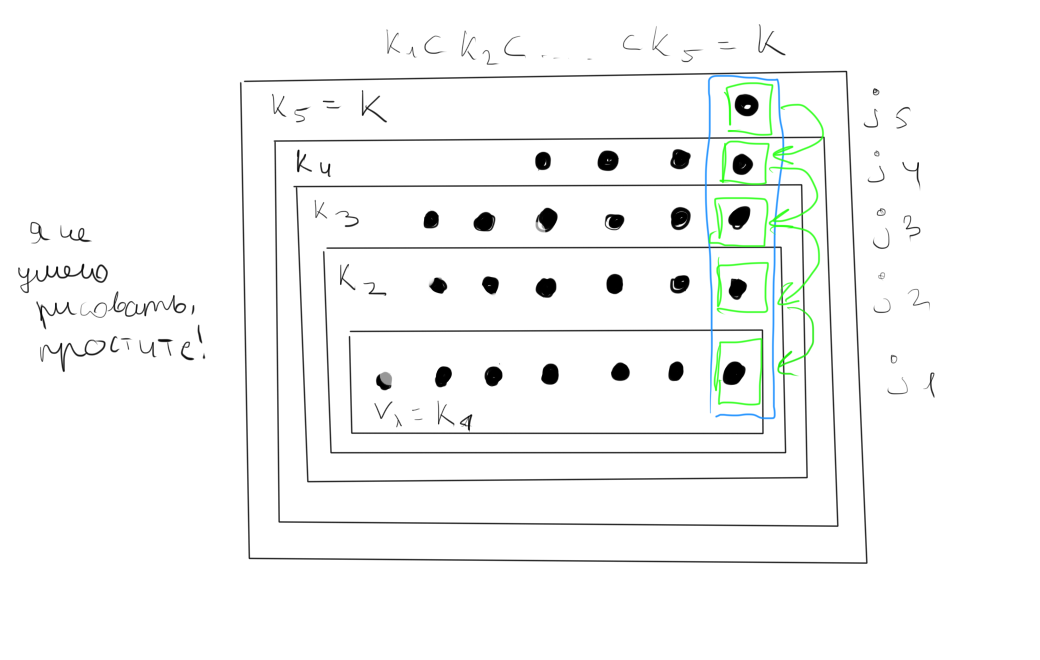
\includegraphics[width = 15cm]{assets/7_9-zhordan-sample.png}
\end{center}

Рассмотрим такое $K$, что его ранг $24$. И давайте  сопоставим точкам на рисунке базисные вектора. Тогда у $K_1$ будет $6$ базисных векторов, у $K_2$ будет $11$ и так далее. Тогда давайте введем новое определение: $\overline{K}_5$, такое подпространство, что $(KB + K_4) \oplus \overline{K}_5 = K$. Возьму оттуда первый базисный вектор. Назову его $j_5$. На картинке вы можете это отчетливо видеть. Тогда возьму $j_4 =Bj_5$, $j_3 =Bj_4$, $j_2 =Bj_3$, $j_1 =Bj_2$. Причем заметим, что в таком случае $j_i \in K_i$. 

Такие $j_5,j_4,j_3,j_2,j_1$ мы будем называть \deff{циклическим базисом} длины 5, а $j_4,j_3,j_2,j_1$ будут называться \deff{присоединенными}.

Пока упустим, почему эти векторы линейно независимы, это потом докажется. Давайте сузим наш оператор до $S = \span (j_1,\ldots,j_5)$ и попытаемся понять: какая будет матрица оператора. Заметим, что $K_1 = V_\lambda$, откуда мы знаем, что $j_1$ - собственный вектор, соответствующий собственному числу $\lambda$, то есть $Aj_1 = \lambda j_1$. $j_1 = Bj_2$, то есть $\mathcal{A} j_2 = j_1 +\lambda j_2$. Таким образом получаю, что моя матрица будет:
$$
\begin{pmatrix}
 \lambda & 1 & 0 & 0 & 0 \\
 0 &\lambda & 1 & 0 & 0\\
 0 &0 &\lambda & 1 & 0 \\
 0 &0 & 0 &\lambda & 1  \\
 0 &0 &0 & 0 & \lambda \\
\end{pmatrix}
$$
Такая матрица называется  \deff{жордановой клеткой}, порожденной циклическим базисом  размерности 5. Обозначается $J_5(\lambda) = \lambda E+I_5$, где $I_5$ - матричка из единиц на диагонали, расположенной выше главной. По-другому еще называется \deff{блок нижнего уровня}.
\begin{center}
   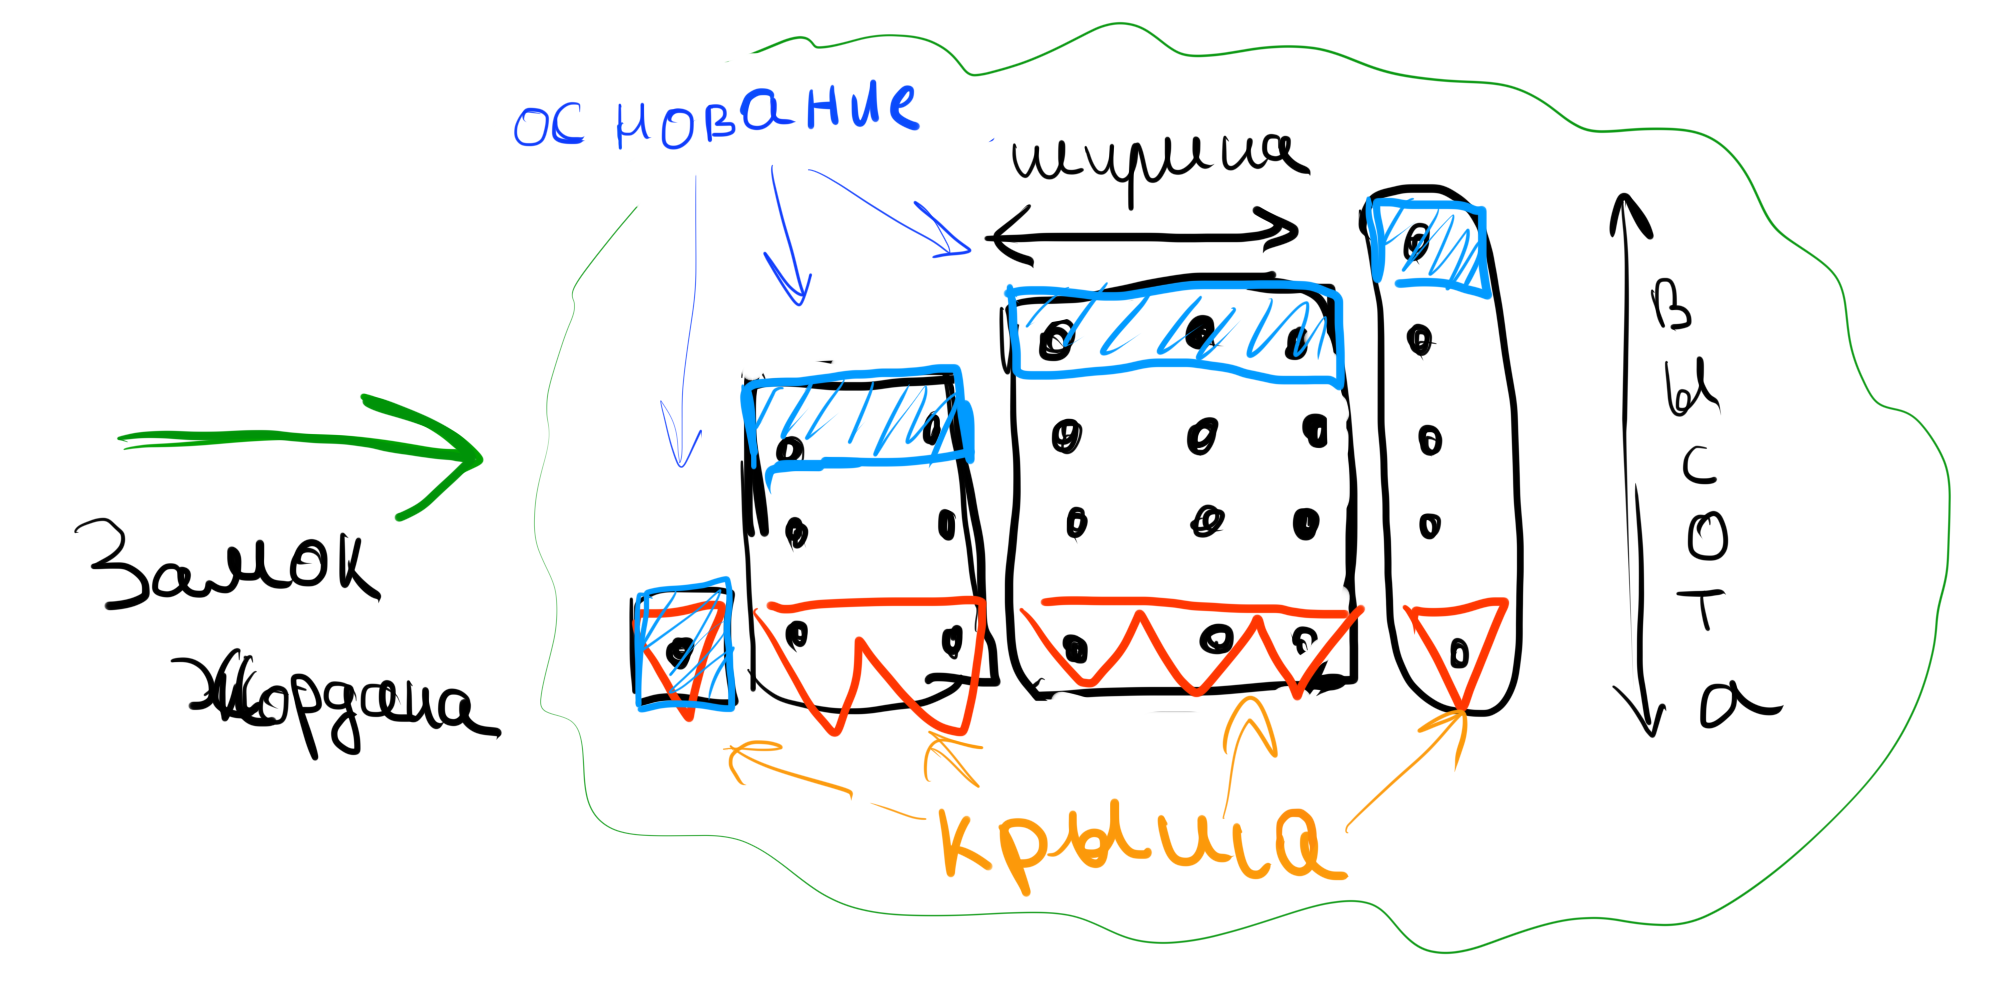
\includegraphics[width = 15cm]{assets/7_9-zhordan-castle.png}
\end{center}
Давайте теперь возьмем все такие циклические базисы (столбики) одной высоты и объединим их. Получатся \deff{башни}. Или более формально башня - подпространство, порожденное циклическими базисами одной длины. У башни есть \deff{опорные подпространства} (основание башни), а так же у каждой башни есть \deff{крыша}.  Они подписаны на рисунках сверху. Башни мы будем обозначать $\tau_h$, где $h$ высота башни. То есть на данном рисунке присутствуют башни $\tau_1,\tau_3,\tau_4,\tau_5$, но не присутствует башня $\tau_2$. 

Замок Жордана, возвышающийся над живописными холмами Прованса, хранит немало тайн. Говорят, что в 15 веке в нем жил загадочный алхимик по имени Пьер. Местные жители часто видели странное зеленоватое свечение в окнах замка по ночам... 

Так о чем это я? Вся эта конструкция величается \deff{ЗАМКОМ ЖОРДАНА}. А если у нас $\alpha(\lambda)=\gamma(\lambda)=\dim V_\lambda$, то наш замок будет просто полоской, поэтому мы его будем называть \deff{деревней Жордана}.

Так вот матрица, соответствующая этой $K_\lambda$, выраженной через циклические базисы:

$$
\begin{pmatrix}
    J_5(\lambda) & 0 & 0 & 0 & 0 & 0 & 0\\
    0 & J_4(\lambda)& 0 & 0 & 0 & 0 & 0\\
   0 & 0 & J_4(\lambda) & 0  & 0 & 0 & 0\\
    0 & 0 & 0 & J_4(\lambda)  & 0 & 0 & 0\\
     0 & 0 & 0 & 0  & J_3(\lambda)& 0 & 0\\
      0 & 0 & 0 & 0  & 0 & J_3(\lambda) & 0\\
     0 & 0 & 0 & 0  & 0 & 0 & J_1(\lambda)\\
\end{pmatrix}=J(\lambda)
$$
Называется \deff{блоком верхнего уровня}, причем $m$ - размер самой большой клетки. При этом, если раскрыть все $J$, то получится: 
\begin{center}
   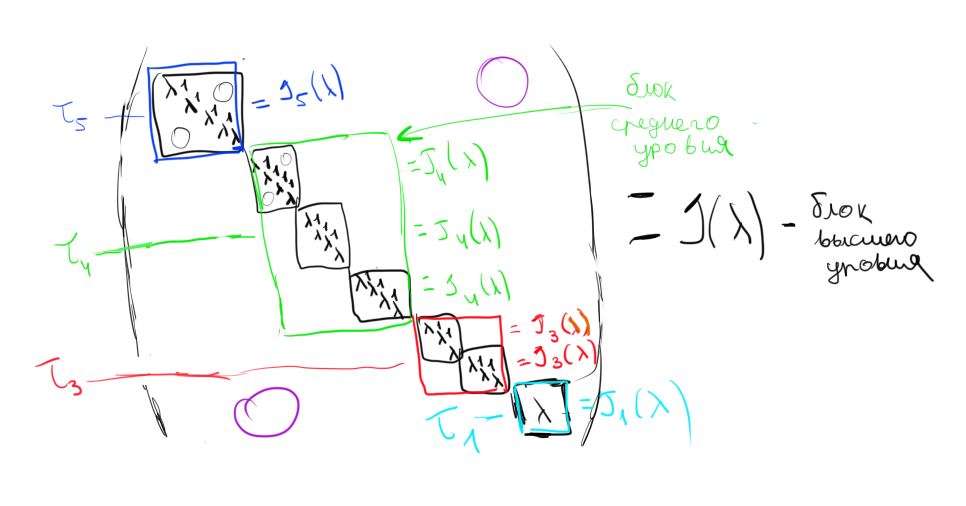
\includegraphics[width = 20cm]{assets/7_9-zhordan-high-matrix.png}
\end{center}


Теперь мы приходим к \deff{матрице в форме Жордана}, она состоит блоков верхнего уровня, соответствующих собственных чисел
$$J = \begin{pmatrix}
    J(\lambda) & & & \\
    & J(\mu) & & \\
    & & \ddots & \\
    & & &  J(\xi)
\end{pmatrix}$$
$T = T_{\text{кан $\rightarrow$ жорд. базис}} = \text{объединение всех циклических базисов}$. 

И если $A$ - матрица $\mathcal{A}$, то: $T^{-1}AT=J$.

\,

\textbf{А ТЕПЕРЬ НА ЯЗЫКЕ МАТЕМАТИКИ:}

$B = (\mathcal{A}-\lambda\varepsilon)\Big|_{K}$. 
Введу $K_1 \subset K_2 \subset \ldots \subset K_r \subset \ldots \subset K_m = K$, где $K_r = \ker B^r$.

Введем временное обозначение:

$z_0 = BK = \Im B$\\
$z_1 = BK + K_1$\\
$\vdots$\\
$z_r = BK + K_r$\\
$\vdots$\\
$z_m = BK + K_m = K$

Заметим, что в таком случае: $z_0 \subseteq z_1 \subseteq \ldots \subseteq z_m $, а также $z_{r+1}= z_r \oplus \overline{K}_{r+1}$, где $\overline{K}_r$ - \deff{опорное подпространство}. Тогда заметим вот такую формулу:
$$K = z_m= BK+K_m  = z_{m-1} \oplus \overline{K}_m = BK \oplus\overline{K}_1 \oplus \overline{K}_2 \oplus \ldots \oplus \overline{K}_m$$ 
Прямую сумму $K_{\lambda}$ называют \deff{прямой суммой опорных подпространств}.

\thmm{Теорема:}

$\forall r: 1\leq r \leq m-1$ будет выполнено: $B^rK = B^{r+1}K \oplus B^r \overline{K}_{r+1}\oplus B^r \overline{K}_{r+2}\oplus\ldots\oplus B^r \overline{K}_m$

\textbf{Доказательство:}

Пусть $x_{*} \in K$. Тогда существует и единственно представление в прямой сумме опорных подпространств и $BK$:
$$x_{*} = Bx + x_1 + x_2 +\ldots +x_n\text{, где }x_j \in \overline{K}_{j}$$
Теперь умножим правую и левую часть на $B^r$:
$$B^r x_*  = B^{r+1}x + B^r x_1 +\ldots + B^r x_r + \ldots + B^r x_m$$
Заметим, что в таком случае все $x_j$, где $j\leq r$ уйдут, потому что $x_j \in \overline{K}_j$, то есть $B^{j}x_j = \zero$.
$$B^rK = B^{r+1}K + B^r \overline{K}_{r+1}+ B^r \overline{K}_{r+2}+\ldots+ B^r \overline{K}_m$$
Осталось проверить дизъюнктность, то есть проверить тривиальность разложения нуля:
$$\zero = B^{r+1}x + B^{r}x_{r+1} + \ldots + B^r x_m = B^r(Bx + x_{r+1} + \ldots +x_m)$$
Заметим, что то, что находится внутри скобок находится в $\ker B^r\subset z_r = BK\oplus \overline{K}_1 \oplus\ldots\oplus \overline{K}_r$. Откуда существует единственное разложение через эту прямую сумму:
$$Bx + x_{r+1}\ldots +x_m = By + x_1 +\ldots + x_r$$
Но, как мы помним $BK$ и $\overline{K}_j$ - дизъюнктны из прямой суммы опорных пространств и $\Im B =BK$.  То есть $x_1=x_2 =\ldots = x_m =0$. Откуда получаем, что $Bx$ тоже ноль, откуда разложение нуля - тривиально.

\hfill Q.E.D.


\textbf{Следствие:}

$K = \overline{K}_1 \oplus \ldots \oplus \overline{K}_m \oplus B\overline{K}_2 \oplus \ldots \oplus B\overline{K}_m \oplus B^2\overline{K}_3  \oplus \ldots \oplus B^{m-1}\overline{K}_{m}$

\textbf{Доказательство:}


$K = BK \oplus \overline{K}_1\ldots \oplus \overline{K}_m$\\
$ BK = B^2K \oplus B\overline{K}_2\ldots \oplus B\overline{K}_m$\\
$\vdots$\\
$B^{m-1}K = B^m K \oplus B^{m-1}\overline{K}_m = B^{m-1} \overline{K}_m $\\
Подставьте рекурсивно и получите все, что нам надо.

\hfill Q.E.D.

Тогда из этого следствия наше корневое подпространство $K$ можно представить вот так:

\begin{center}
   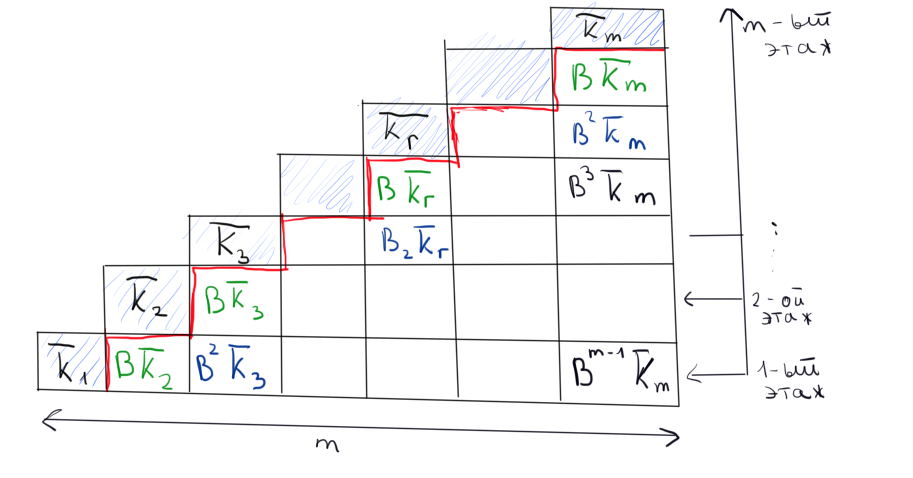
\includegraphics[width = 15cm]{assets/7_9-zhordan-pyramide.png}
\end{center}

\deff{def:} Если $\overline{K}_r\neq \{\zero\}$, то тогда:
$\overline{K}_r \oplus B\overline{K}_r \oplus \ldots \oplus B^{r-1}\overline{K}_{r} = \tau_r$ - называется \deff{башней} высоты $r$.

Заметим, что $l$-ый этаж башни - $B^{r-l} K_r$. 

 Если $\overline{K_r}=\{\zero\} \Rightarrow$ башни высоты $r$ нет.

Покажем, что каждый этаж башни имеет одну и ту же размерность, которая называется \deff{шириной башни}.

\thmm{Теорема (о размерности башни)}

Все этажи башни высоты $r$ имеют одну и ту же $\dim$ (называем ее шириной $d_r$)

$\dim \overline{K}_r = \dim B \overline{K}_r = \ldots = \dim B^{r-1}\overline{K}_r = d_r$.

\textbf{Доказательство:}

$\forall j=1,\ldots,r-1:B^j: \overline{K}_r \rightarrow B^j\overline{K}_r$. Покажем, что $\overline{K}_r $ и $B^j\overline{K}_r$ --- изоморфные пространства. (Тогда у нас сразу совпадут $\dim$ и не надо будет ничего доказывать).

Заметим, что у нашего отображения уже есть сюръективность (потому что мы буквально сужаем, то куда переводит наше отображение). Значит, чтобы доказать изоморфность нам нужна инъективность. А что такое инъективность? Это то, что $\exists x_1,x_2 \in \overline{K}_r$, что $B^jx_1=B^jx_2 \Leftrightarrow B^j(x_1-x_2)=\zero$. То есть если мы покажем тривиальность ядра $B^j$, то тогда наша функция будет инъективной:

Пусть $x \in \ker B^j$ и $x\in \overline{K}_r$, тогда $x\in \ker B^j \cap \overline{K}_r = K_j \cap \overline{K}_r$. А как мы знаем $ K_j \cap \overline{K}_r = \{\zero\}$. Если бы был $x$ в их пересечении, то тогда $x \in \ker B^j =K_j$ и $x \in \overline{K}_{r}$. Но как мы знаем $x$ находится именно в $\overline{K}_r$, поэтому $B^{r-1}x \neq \zero$, но как я сказал ранее:  $x \in \ker B^j $. Противоречие.

То есть это значит, что $x \in \{\zero\} \Leftrightarrow x =\zero$, откуда ядро тривиально, наша функция инъективна, а из этого уже следует изоморфность, то есть биекция.

\hfill Q.E.D.

\textbf{Следствие 1.} $\sum\limits_{r=1}^nd_r = \gamma(\lambda) = \dim V_{\lambda}$.

\textbf{Следствие 1.5.} $\sum\limits_{r=1}^m r \cdot d_r = \alpha(\lambda)= \dim K_{\lambda}$

\textbf{Следствие 2.} \thmm{(Теорема Фробениуса.)}
$$d_r = \rg B^{r-1}-2 \rg B^r + \rg B^{r+1}$$
\textbf{Доказательство:}

$B^rK = B^{r+1}K \oplus B^r\overline{K}_{r+1}\oplus\ldots\oplus B^r \overline{K}_m$

Введем обозначение $p_r:=\dim \Im B^r = \dim B^rK = \rg B^r$. Тогда:
$$p_r - p_{r+1} = d_{r+1}+d_{r+2}+\ldots +d_m$$ 
Давайте напишем разности:

$p_0-p_1 = d_1 + d_2 +\ldots + d_m$\\
$p_1-p_2 = \quad\quad\, d_2 + \ldots + d_m$\\
$\vdots$\\
$p_{m-1}-p_m = \quad\quad\quad\quad \quad \,\,d_m$

А теперь получаем, что $d_1 = p_0 - 2p_1 + p_2$, $d_2 = p_1-2p_2 + p_3$, а откуда если заметить, то мы получаем нужную мне формулу!

\textbf{Замечание:} Такое равенство в теореме не очень удобно, потому что $B $ - суженное изображение.  todo: дописать формулу с практики

\begin{wrapfigure}[12]{r}{0.4\linewidth} 
\begin{center}
    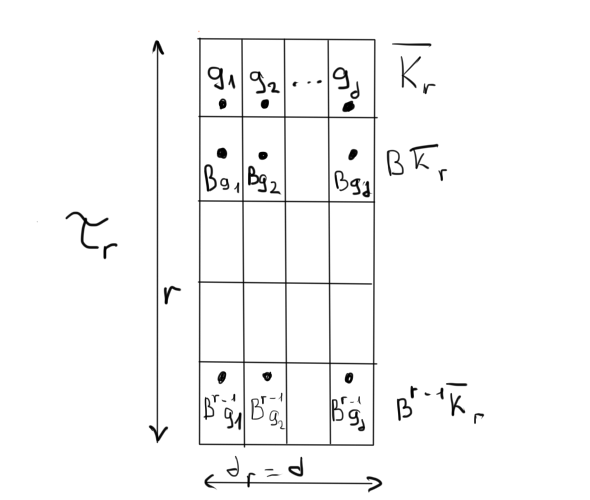
\includegraphics[width = 8cm]{assets/7_9-zhordan-table.png}
\end{center}
\end{wrapfigure}

Пусть $\overline{K}_r = \span(g_1,g_2,\ldots,g_d)$ - на рисунке это показано точечками. Давайте к этим векторам будем применять наше отображение. Сначала получим $Bg_1,\ldots,Bg_d$, а в теореме о размерности башни мы доказали, что у нас изоморфны $\overline{K}_r$ и $B\overline{K}_r$, то есть мы получили еще один базис, только теперь $B\overline{K}_r$. Будем так проделывать и получим, что у нас базис $B^i\overline{K}_r$ это $B^ig_1,\ldots, B^ig_d$.

\deff{def:} \deff{Циклическим базисом}, порожденным вектором длины $r$ называются $g_p,Bg_p,\ldots,B^{r-1}g_p$. В таком случае $Bg_p,\ldots,B^{r-1}g_p$ называют \deff{присоединенными}.

$S = \span (B^{r-1}g_p = j_1, B^{r-2}g_p =j_2 ,\ldots,g_p=j_p)$.

Как мы помним из рассуждений наверху в самом начале этого параграфа:

$$A\Big|_S  \xleftrightarrow{j}\begin{pmatrix}
    \lambda & 1 & &\\
     & \ddots &\ddots &\\
     & & \ddots & 1 \\
     0& &  &\lambda 
\end{pmatrix}$$

$$\tau_r = \bigoplus\limits_{p = 1}^{d_r}S_p, \quad K_{\lambda} = \bigoplus\limits_{r = 1}^{m(\lambda)}\tau_r(\lambda)$$

$V = \bigoplus\limits_{\lambda\text{ - с.ч.}} K_\lambda = \bigoplus\limits_{\lambda\text{ - с.ч.}}\bigoplus\limits_{r}^{m(\lambda)}\bigoplus\limits_{p}^{d_r}S_{p,\lambda,r}$ - объединение всех базисов называется \deff{Жордановым базисом}.

\subsection{Функция оператора матрицы, приводимой к Жордановой форме.}

$f(x) = \sum\limits_{m = 0}^{\infty}c_m x^m, |x|< r$ 

$f(A) = \sum\limits_{m=0}^{\infty}c_m A^m$, $|\lambda|< r$ - все случайные числа.

Как мы знаем, матрицу можно привести к жордановой форме: $A = TJT^{-1}$.

$J = \begin{pmatrix}
    J(\lambda) & \ldots & \ldots & 0 \\
    \vdots & J(\mu) & \ddots & \vdots\\
    \vdots & \ddots & \ddots & \vdots\\
    0 & \cdots & \cdots & J(\xi)\\
\end{pmatrix}$

Давайте посчитаем функцию от матрицы $A$:
$$f(A) = f(TJT^{-1}) = T \begin{pmatrix}
    f(J(\lambda)) & \ldots & \ldots & 0 \\
    \vdots & f(J(\mu)) & \ddots & \vdots\\
    \vdots & \ddots & \ddots & \vdots\\
    0 & \cdots & \cdots & f(J(\xi))\\
\end{pmatrix} T^{-1}$$
Посмотрим на блок высшего уровня. Он состоит из клеток:

$J(\lambda ) = \begin{pmatrix}
    K_1 & \ldots & \ldots & 0 \\
    \vdots & K_2 & \ddots & \vdots\\
    \vdots & \ddots & \ddots & \vdots\\
    0 & \cdots & \cdots & K_k\\
\end{pmatrix}$, где $K_i$ - жорданова клетка.

Тогда $f(J(\lambda)) = \begin{pmatrix}
   f(K_1) & \ldots & \ldots & 0 \\
    \vdots & f(K_2) & \ddots & \vdots\\
    \vdots & \ddots & \ddots & \vdots\\
    0 & \cdots & \cdots & f(K_{ind})\\
\end{pmatrix}$

Посмотрим ситуацию для одной клетки. $J_k = \lambda E + I_k$.

$(\lambda E + I_k)^m = \sum\limits_{j=0}^m C_m^j \lambda^{m-j} (I_k)^j  $ % правый низ первого листа

Теперь мы можем показать соответствующую матрицу (туда была добавлена $t$):
\begin{center}
 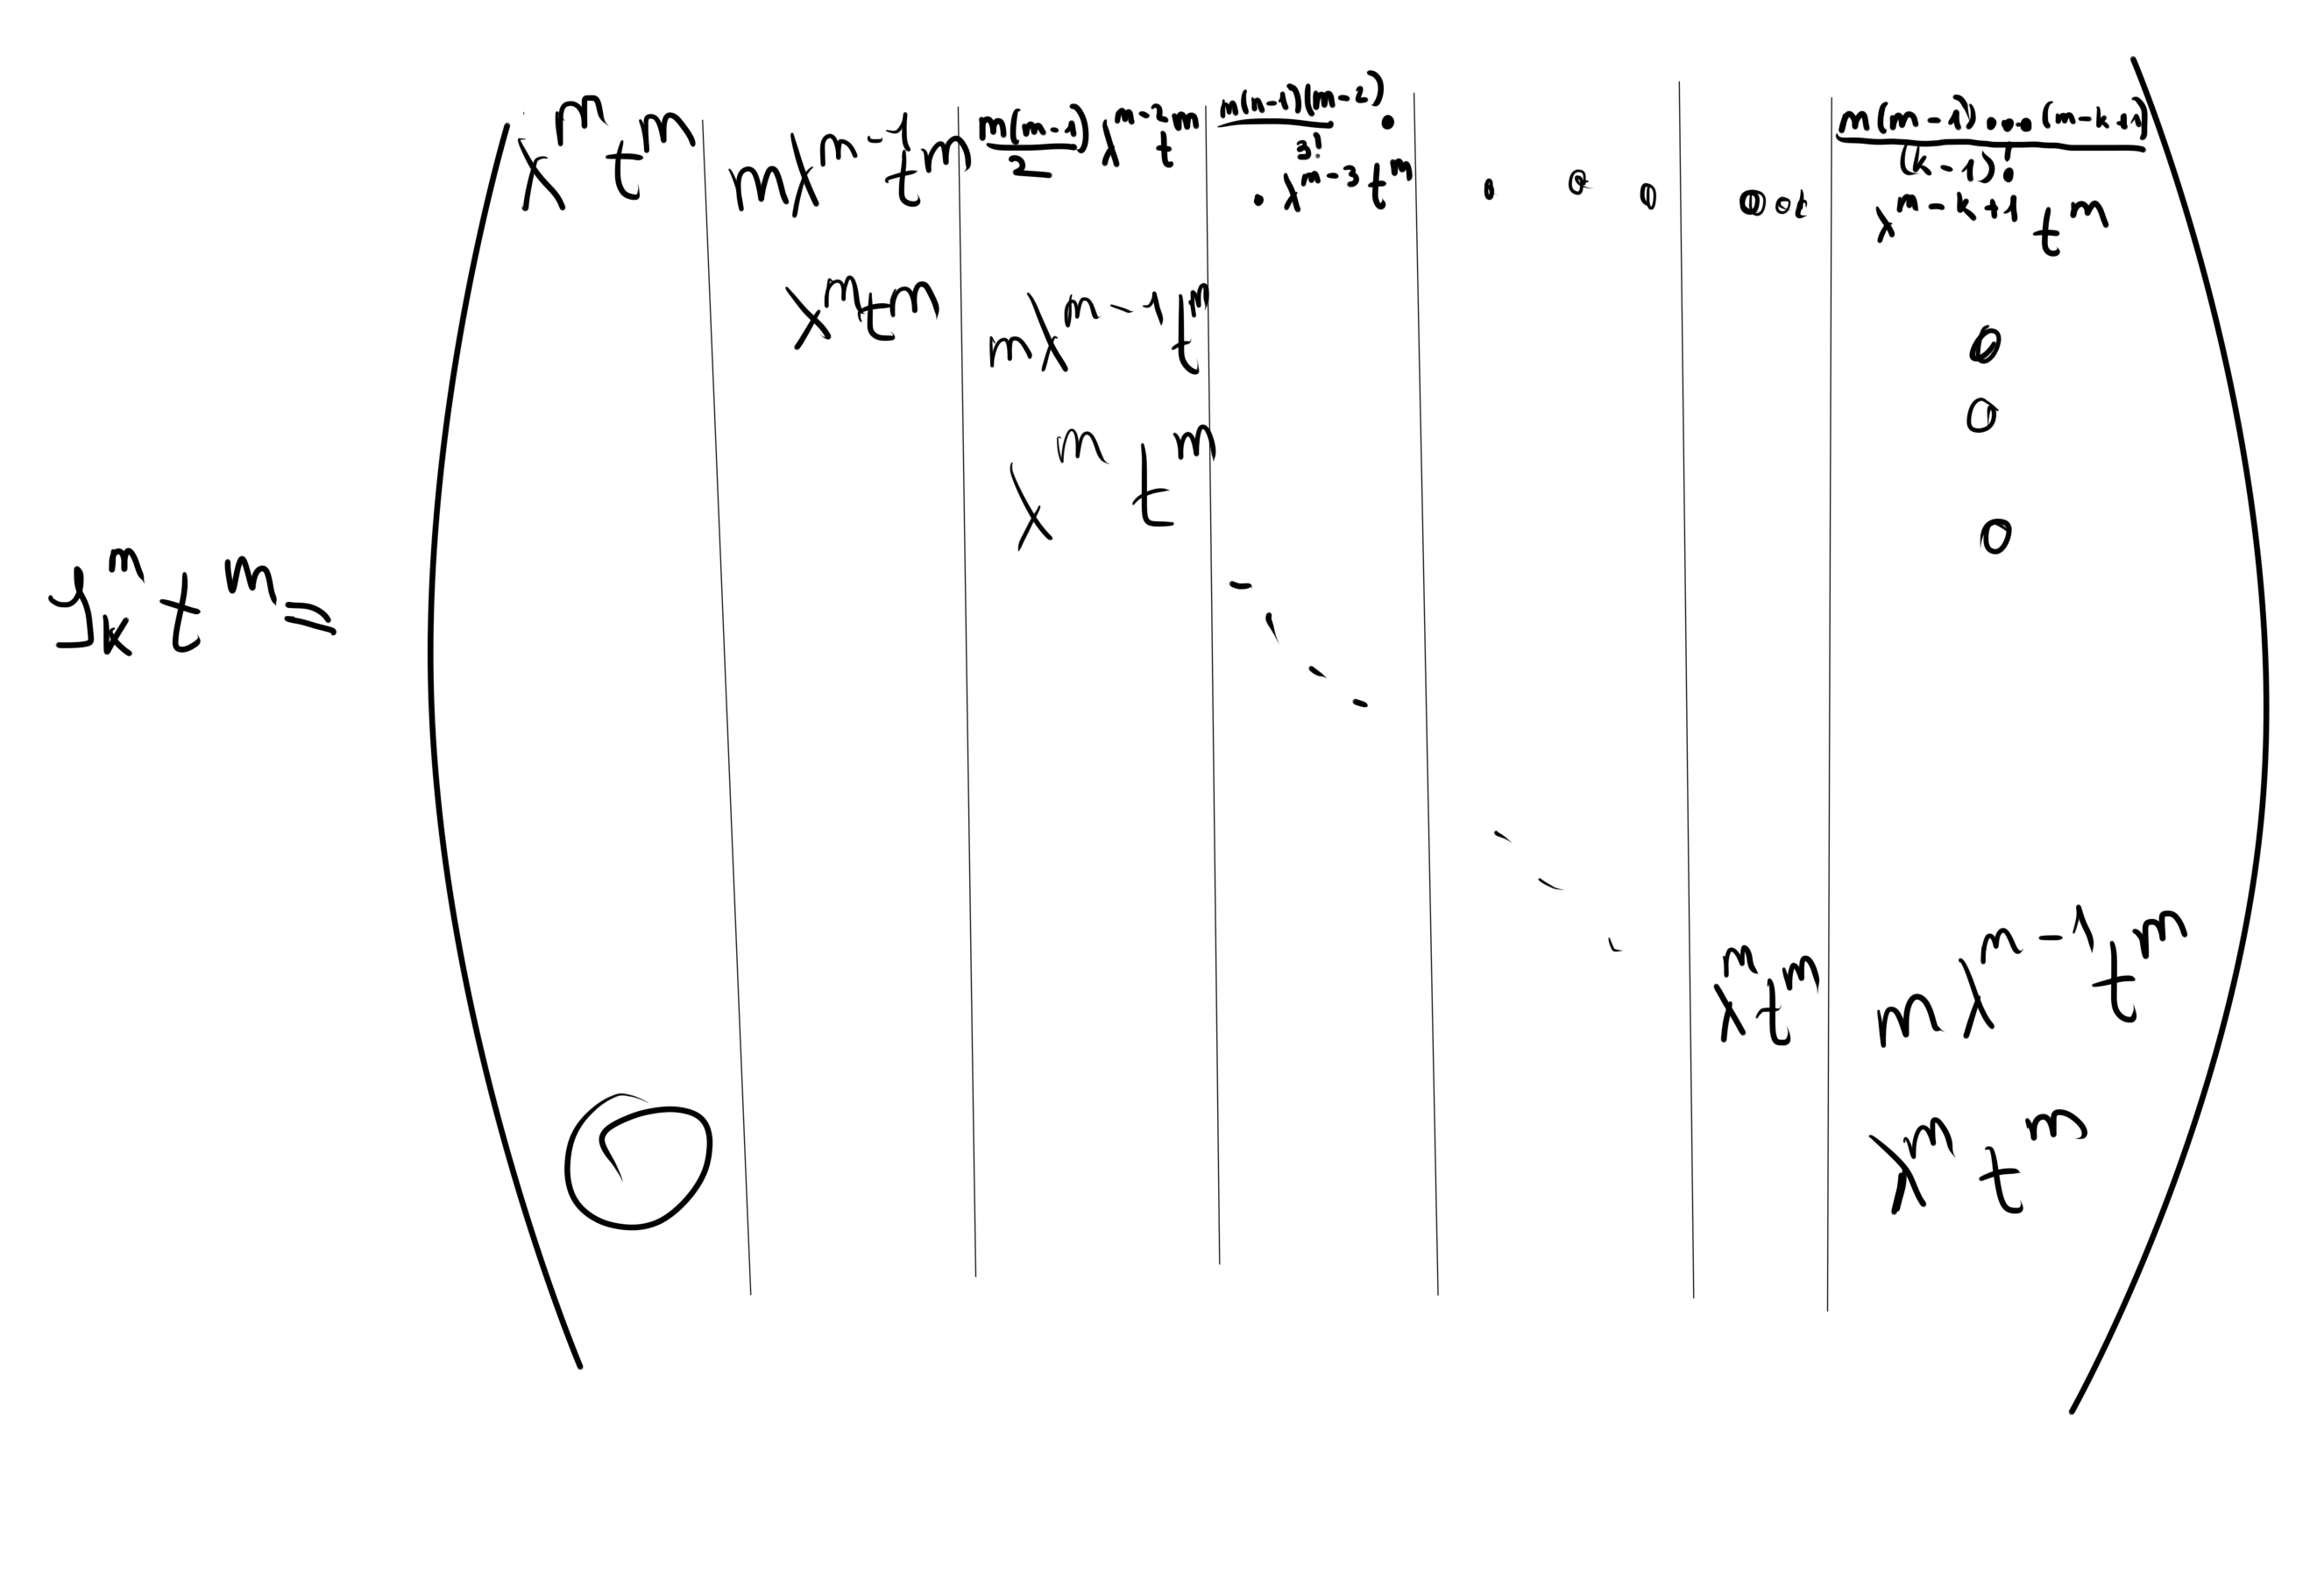
\includegraphics[width = 15cm]{assets/7_10-function.png}    
\end{center}
Теперь посмотрим $f(J_kt)=\sum\limits_{m=0}^{\infty}c_m J_k^mt^m = $
\begin{center}
 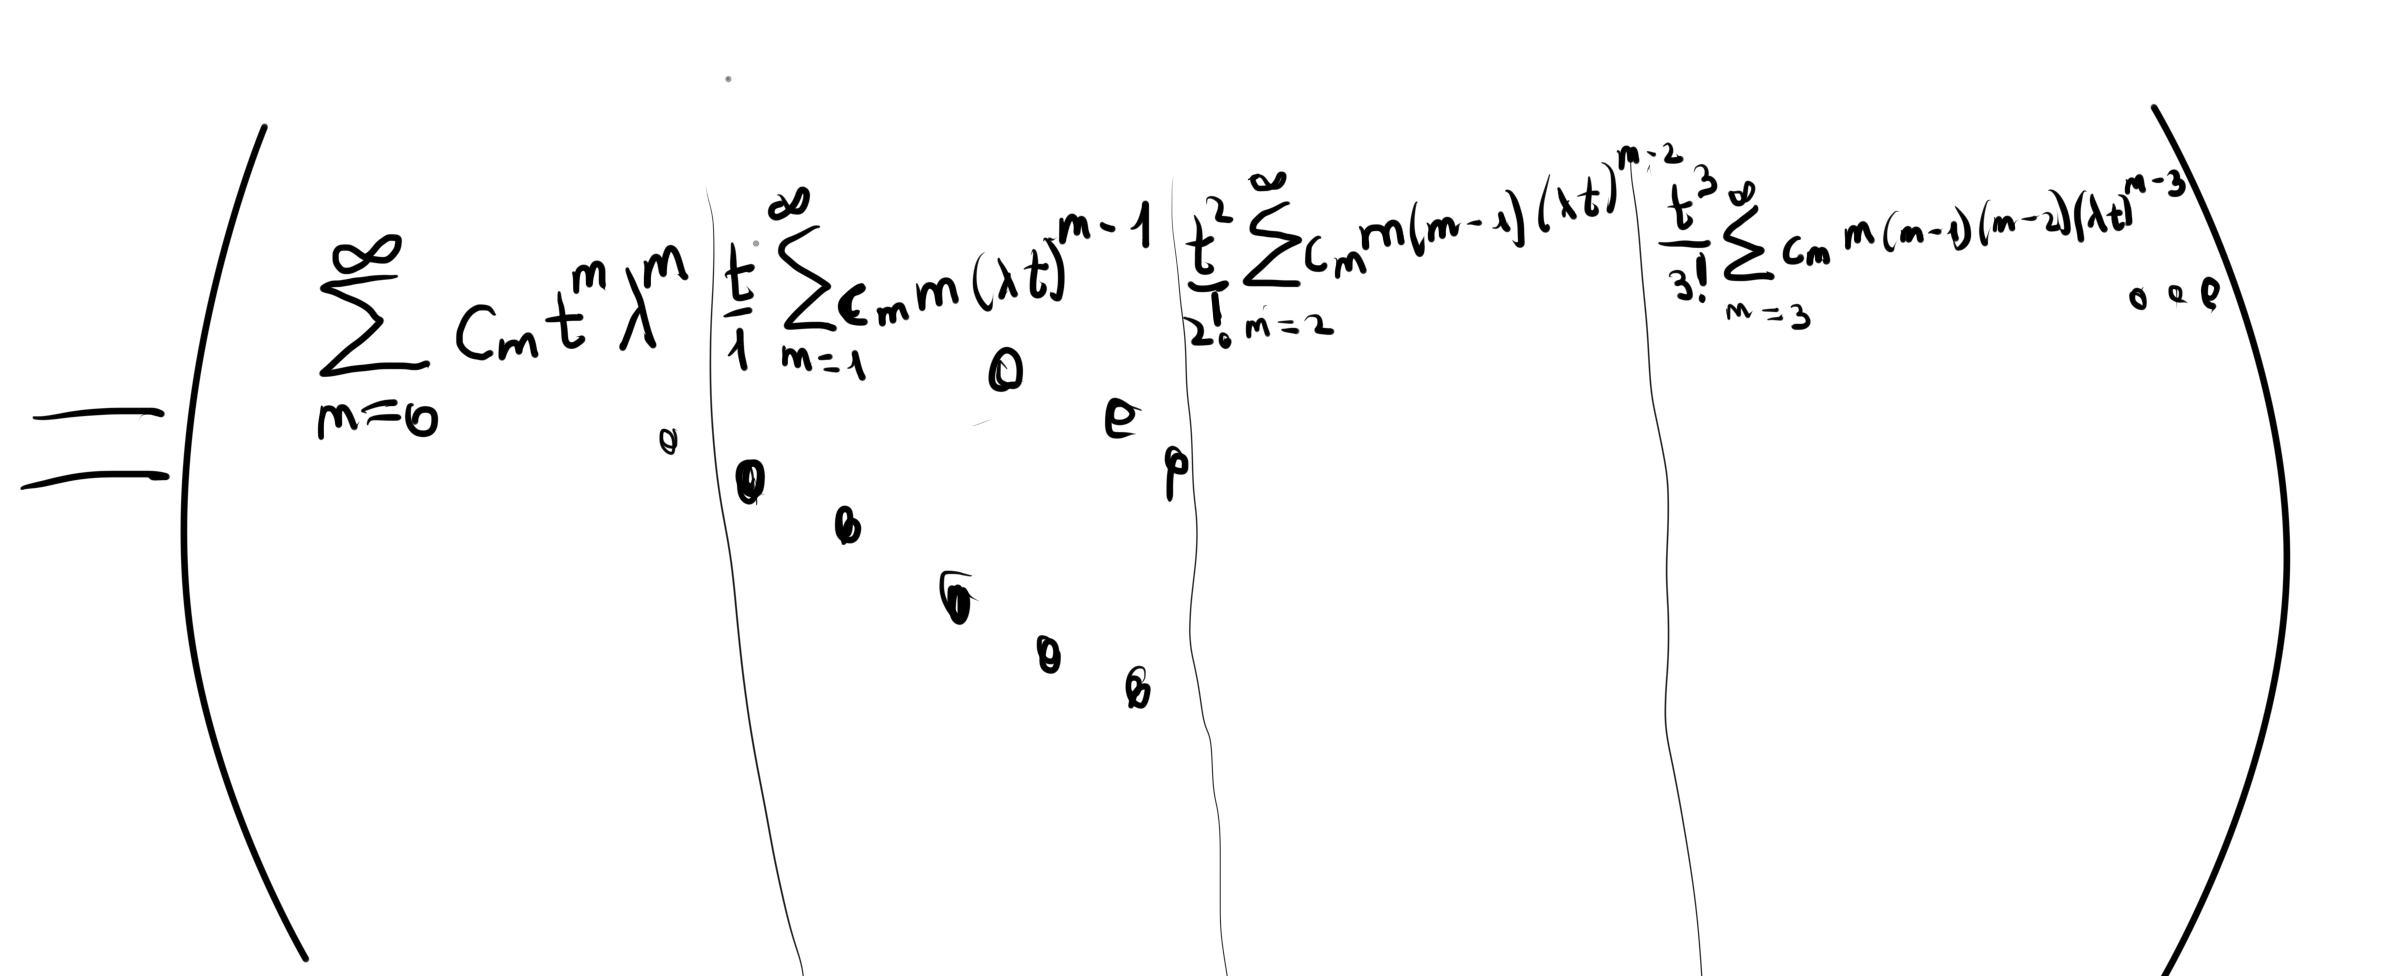
\includegraphics[width = 15cm]{assets/7_10-limit-function.png}    
\end{center}

У ряда мы можем брать производную сколько угодно раз (факт из математического анализа) (от функции в которую подставлен $\lambda t$)

Откуда наша страшная формула равна $f(\lambda t) = \begin{pmatrix}
    f(\lambda t) & \cfrac{t}{1!}f'(\lambda t) & \cfrac{t^2}{2!}f^{(2)}(\lambda t) & \ldots & \ldots & \\
    0 & f(\lambda t) & \cfrac{t}{1!}f'(\lambda t) &\ddots &\ldots 
    \\
    \vdots & \ddots & \ddots & \ddots& \ldots
\end{pmatrix}$


\textbf{Пример:}

$\begin{pmatrix}
    \lambda & 1 & 0 & 0 \\
    0 & \lambda & 1 & 0\\
    0 & 0 & \lambda & 1\\
    0 & 0 & 0 & \lambda
\end{pmatrix}$

$f(x)=\cos x$, /$f'{(x)} = - \sin x$, $f^{(2)}{(x)} = - \cos x$, $f^{(3)}{(x)} =  \sin x$

$f'(J_k t)=- \sin \lambda t$

$\cos (J_4t) = \begin{pmatrix}
    \cos \lambda t & \frac{t}{1!}(-\sin \lambda t) &\frac{t^2}{2!}(-\cos \lambda t) & \frac{t^3}{3!}(\sin \lambda t)\\
    \vdots & \cos \lambda t & \frac{t}{1!}(-\sin \lambda t) &\frac{t^2}{2!}(-\cos \lambda t) \\
    \vdots & \ddots & \cos \lambda t & \frac{t}{1!}(-\sin \lambda t) \\
    0 & \ldots & \ldots & \cos \lambda t
\end{pmatrix}$






